% REMEMBER: You must not plagiarise anything in your report. Be extremely careful.

\documentclass{l4proj}

    
%
% put any additional packages here
%

\begin{document}

%==============================================================================
%% METADATA
\title{Level 4 Project - Virtual Turing Tumble}
\author{Luke Gall, 2298070g}
\date{September 14, 2018}

\maketitle

%==============================================================================
%% ABSTRACT
\begin{abstract}
    Every abstract follows a similar pattern. Motivate; set aims; describe work; explain results.
    \vskip 0.5em
    ``XYZ is bad. This project investigated ABC to determine if it was better. 
    ABC used XXX and YYY to implement ZZZ. This is particularly interesting as XXX and YYY have
    never been used together. It was found that  
    ABC was 20\% better than XYZ, though it caused rabies in half of subjects.''
\end{abstract}

%==============================================================================

% EDUCATION REUSE CONSENT FORM
% If you consent to your project being shown to future students for educational purposes
% then insert your name and the date below to  sign the education use form that appears in the front of the document. 
% You must explicitly give consent if you wish to do so.
% If you sign, your project may be included in the Hall of Fame if it scores particularly highly.
%
% Please note that you are under no obligation to sign 
% this declaration, but doing so would help future students.
%
\def\consentname {Luke Gall} % your full name
\def\consentdate {12 February 2021} % the date you agree
%
\educationalconsent


%==============================================================================
\tableofcontents

%==============================================================================
%% Notes on formatting
%==============================================================================
% The first page, abstract and table of contents are numbered using Roman numerals and are not
% included in the page count. 
%
% From now on pages are numbered
% using Arabic numerals. Therefore, immediately after the first call to \chapter we need the call
% \pagenumbering{arabic} and this should be called once only in the document. 
%
% Do not alter the bibliography style.
%
% The first Chapter should then be on page 1. You are allowed 40 pages for a 40 credit project and 30 pages for a 
% 20 credit report. This includes everything numbered in Arabic numerals (excluding front matter) up
% to but excluding the appendices and bibliography.
%
% You must not alter text size (it is currently 10pt) or alter margins or spacing.
%
%
%==================================================================================================================================
%
% IMPORTANT
% The chapter headings here are **suggestions**. You don't have to follow this model if
% it doesn't fit your project. Every project should have an introduction and conclusion,
% however. 
%
%==================================================================================================================================
\chapter{Introduction}

% reset page numbering. Don't remove this!
\pagenumbering{arabic}

\section{Motivation}
Turing Tumble, a marble based board game is designed to teach children and adults the logic found within a computer chip. It focuses on teaching 6 basic logical components that can be used to build up powerful computational patterns capable of storing state, activating conditionals, and counting in binary. The game uses puzzles and gamification to provide an assessable and fun environment for users to learn how small, simple components can be combined to produce powerful results. With puzzles included to provide external learning motivation for players it succeeds in creating an interactive and addicting learning environment that can help improve users knowledge of the inner workings of computers as well as develop practical skills in logic based problem solving. 

The board game, primarily focused on being a fun learning tool for children, is also interesting enough to warrant the attention of adults and students. It is designed to be Turing complete, allowing users to build patterns with the same computational expressiveness as a modern day computer. With this computational expressiveness contained within simple marbles, mechanical pieces, and a board the game can be of interest to students wanting to explore a fun and unique way to compose computationally powerful patterns.  

A simulation of the game gives an easy and accessible tool to play and learn using a Turing Tumble. This project focuses on the creation of a faithful Turing Tumble simulator while adding features focused on improving learning through the game. The main aim was creating an easy to use tool for users unfamiliar with the physical board game rather than adding new complex features to the game. This allows new users to learn and play the game using the simulation while ensuring unnecessary complexity isn't added. 


\section{Goals}
\textbf{Simulate a Turing Tumble board} The main goal of the program to correctly simulate all logical configurations that are possible on a physical version of the Turing Tumble board. This is required to ensure a faithful simulation is created for users to use as a replacement for the physical board game. This includes ensuring that all pieces follow the exact logic of the game board and the simulation can play through a series of marbles going down the board and recording the result. The marble correctly following the path determined by the pieces is an important aspect for a user to learn and understand how a combination of small but powerful pieces can lead to complex results. Marbles must also be recorded when they reach the bottom of the board. It is important that users can see the marbles collected as this is an essential result used to understand the output of the Turing Tumble board, including patterns expected in puzzles. It was decided that the board created in the program should follow the exact size and specifications of the physical board to keep a faithful simulation while avoiding unnecessary complexity for new users to the game.

\textbf{User can build their own Turing Tumble configuration} User must be able to select and place the 6 logical pieces onto the various slots of a Turing Tumble board. This will allow users to create and then simulate different combinations of pieces on the board, allowing them to learn the power of the board by creating their own individual configurations. It was decided that the users should be able to place pieces using a on screen board to provide an easy and efficient way to create new combinations. While a txt file could be used to input the different pieces, however this was seen as time consuming for the user and would lead to extra complexity required to validated this input. 

\textbf{Increase learning via puzzles} Users should be able to view and play puzzles from a selection included with the official Turing Tumble game guide. The game while interesting in it's own right for users interested in building complex patterns using simple components, is more enjoyable and motivating for new users by providing a set of puzzles designed to teach the various aspects of the board and display the computational power available. The user should have a clear set of puzzles they can work through with difficulty increasing at a steady pace to keep motivation high and the challenge steady to improve the user's learning experience. The puzzles can be used to teach how a Turing Tumble works as well as improve logical problem solving skills.    

\textbf{Should be easy to use and understand} The target audience of this program is Computer Science students interested in the game and school pupils that could use this program as a replacement for the physical board game. This means that the program should be easy to use and understand for users unfamiliar with the Turing Tumble game. It is important that users can focus on how the board works and what they can learn from it rather than getting confused or disinterested because the program is hard to understand or follow. 

\textbf{Puzzle ecosystem} To increase the likelihood that users are encouraged to use the site more than once it should be possible for users to create their own puzzles and upload them to the site. By allowing users to create their own puzzles they will learn more about creating logical challenges while also encouraging other users to play these puzzles and learn more using the game. This ecosystem can ensure that the user has multiple reasons to continue using the site after completing the original set of puzzles. This is important as it would encourage more time spent with the game, increasing the likelihood of users learning more about inner workings of computers as well as logical problem solving skills. 

%==================================================================================================================================
\chapter{Background}
\section{Turing Tumble}
\label{section:background}

The Turing Tumble is a marble based board game that was designed to teach children the power of small simple components and how they can be connected together to produce algorithms capable of computationally powerful results. A picture of the board can be found in \ref{fig:ttboard}, two marble dispensers are located in the top two corners of the board, one for blue and another for red marbles. Each marble represents 'electricity' in the computer metaphor that persists through the board. A marble travels down the board interacting with various pieces that represent different computer components. At the bottom of the board it will flip either a blue or red flipper which will release another marble of that colour. The marble is also stored and displayed at the bottom. The board is filled with a criss cross pattern of Pins and Component Slots, all 6 pieces fit in \emph{Component Slots}, while only the Gear piece fitting in \emph{Pins}. Each piece has it's own logic that will change the direction of a marble going down the screen. The 6 pieces are described below.

\textbf{Ramp}
The Ramp component is the simplest component and acts as a 'wire' in the computer metaphor that persists throughout the components. The Ramp sends a marble either right or left depending on the direction the curved end is facing. As the marbles aren't allowed to drop freely until they reach the end, the ramp is the most common way to direct the marbles to the desired location.

\textbf{Crossover}
The Crossover is a non reversible piece that continues the direction a marble is travelling into the component and allows the marbles to enter from either side.This piece is metaphorically equivalent to wires crossing over in chips, it allows paths created using ramps and other components to cross over each other.

\textbf{Bit}
The Bit component acts as a metaphorical switch that will change the direction the next marble will travel based on if it is 'on' (pointing to the right) or 'off' (pointing to the left). It sends marbles in the opposite direction it is facing. When a marble passes through a Bit it changes the direction of the piece. These components can be used to represent registers that store binary represented values.

\textbf{Interceptor}
This component catches a marble and stops the execution of the Turing Tumble as the marble will no longer be able to reach the end of the board and release another marble. This component is similar to a shutoff switch inside a regular computer. 

\textbf{Gear}
Gears are the only components that can be placed on Pins on the board and act as connections between a number of gear bits. They turn either 90° left or right. 

\textbf{Gear Bit}
This component is a like a Bit in that it stores state by pointing left or right and will send a marble in the opposite direction it is facing and then change direction. A Gear Bit not connected to a Gear will act and behave exactly like a normal Bit component. When a Gear Bit changes direction it will also turn any connecting gears which in turn will change the direction of any other Gear Bits and so on. The combination of this component and the Gear is claimed to make the game 'Turing Complete'.

Using a combination of gear and gear bits we can make new logical components like latches, fixed position switches, set switches and flip flops.

\begin{figure}
    \centering
    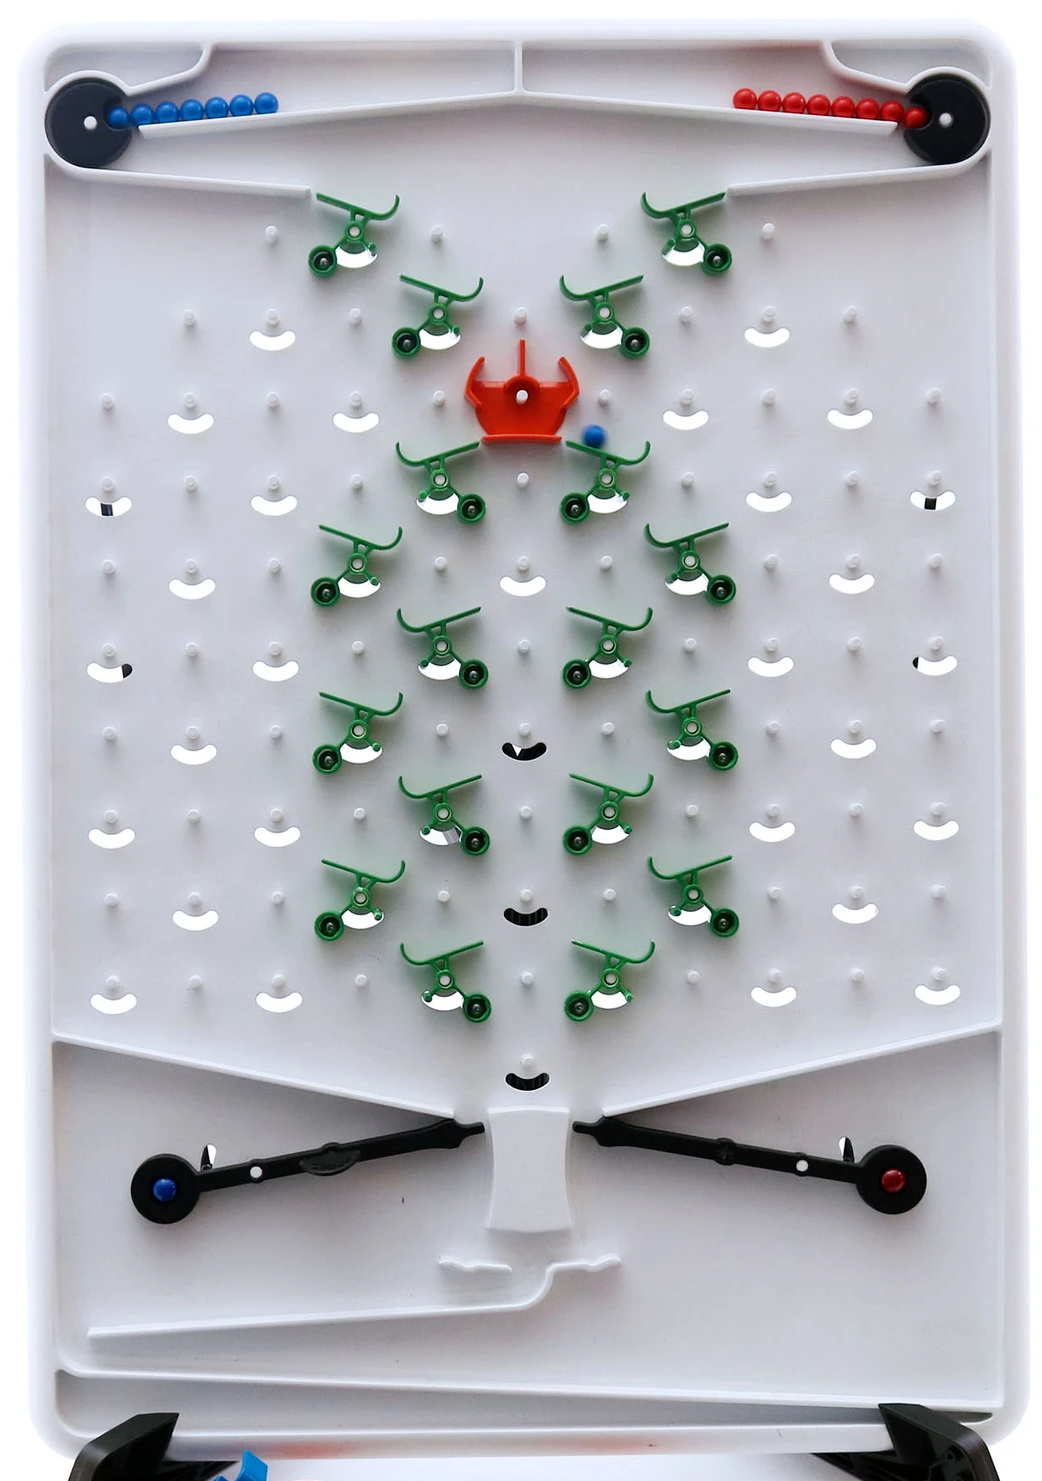
\includegraphics[width=0.5\linewidth]{images/turingTumbleBoard.png}
    \caption{A physical Turing Tumble board with pieces placed onto the board. The marble dispensers are at the top left and right corners with the flippers at the bottom. The boards design is implemented in this program. This image was obtained from (\cite{turing_tumble_picture}).}
    \label{fig:ttboard}
\end{figure}


\section{Existing Simulations}
Research was carried out into existing simulations of the Turing Tumble and evaluation was carried out.

\subsection{Overview}
Various simulations of the Turing Tumble exist online or as downloadable programs. Three such programs were explored and analysed. A paid version was found that implements the board in virtual reality but as this product and implementation style would be unaccessible for the majority of the target audience it was not evaluated. The products were analysed based on the goals set for the project and helped define the requirements for the program.

\subsection{Turing Tumble Simulator}
Turing Tumble Simulator is an open source simulator running in a web browser and hosted on Github pages. (\cite{turing_tumble_simulator}). It was created in Typescript using Javascript libraries for graphics and gravity simulation. 

\textbf{Advantages}
\begin{itemize}
    \item The gravity simulation is impressive and gives a clear and intuitive simulation of the logic of a physical Turing Tumble board. Including when marbles fall and interact with the different pieces.
    \item Marbles are simulated correctly when falling down the board and allow complicated patterns to be simulated.
    \item Extra marbles can be easily added to the dispensers and are collected at the bottom of the board. Unlike other simulators where the number of marbles is represented by numbers, in this implementation it is clearly represented by a graphic for each marble in the dispenser, similar to how it would look it the physical board game.
    \item A tutorial page has been added to give clear descriptions of how the pieces and the application works.
    \item The board can be made larger and edited by adding new walls, slots, dispensers, and flippers giving a large amount of possible customisation options to making complicated patterns for the board. This can allow users to fully explore the computational power of the Turing Tumble giving more space to add complex patterns.
    \item The board has different speed options to control the speed of the marble falling down the board, helpful to improve user understanding of how the pieces are interacting with the marble.
    \item An option to change the graphical representation of the pieces can be activated to change the pieces into a simpler view, in which the pieces are represented by a simple graphic showing the direction the marble can go.
    \item Can download a board as an image, which can later be uploaded to the site. This is an unusual implementation of saving boards where normally a text file is used but the image allows the saved version to be easily recognisable.
\end{itemize}

\textbf{Disadvantages}
\begin{itemize}
    \item Only two pages on the simulation with no clear direction for a new user unfamiliar with a Turing Tumble. This can lead to some initial confusion to a user unfamiliar with what a Turing Tumble is and why they should be interested.
    \item No puzzles can be played on the simulation. This can lead to a lack of an external motivator for users to play with the simulation instead relying on them needing an internal motivator of wanting to learn the Turing Tumble without prompt.
    \item To change the direction of a piece, a user must first place a piece then select the 'hand' tool to click on this piece to change it's direction. It is unclear why the hand tool would be necessary to change the direction of a piece while also being inefficient to change the direction of newly placed pieces.
    \item Too many marbles collected at the bottom can lead to marbles overflowing on top of each over reducing clarity to the order of marbles collected by the board.
    \item The tutorial page doesn't describe how a Turing Tumble board works and may be insufficient for a user unfamiliar with the game to understand.
    \item Can't step through a marble path or pause the marble going down the screen so users would need to use the slowest speed to aid understanding of the exact marble path.
    \item Marbles can drop from any height and reach the end of the board and trigger a new marble going against the rules of the physical Turing Tumble.
\end{itemize}

\textbf{Overall}
A very visually appealing simulation that very faithfully simulates how a physical game would play out by integrating complex gravity simulation. The site can be difficult to understand without having previous experience with a Turing Tumble and no puzzles can be played by users, meaning only an internal motivator of an interest in the Turing Tumble can motivate users to use the site.

\subsection{JS Tumble}
JS Tumble is a Javascript emulator that simulates a Turing Tumble board and is available online \cite{jstumble}.

\textbf{Advantages}
\begin{itemize}
    \item The simulator correctly simulates all pieces of the Turing Tumble board and has a clear graphic for all pieces.
    \item Pieces can be easily placed using a click and place system, with a held piece indicated by a red outline on the selection bar.
    \item A small tutorial text box can be obtained that gets a short description of the board and how to run the simulation. This tutorial is helpful in given users a brief understanding of how to use the various parts of the page.
    \item Users can send the current board pattern to others by sharing a URL with the current board set up. This is useful in helping to foster a community of people to share puzzles with.
    \item Tooltips appear when hoovering over options to give a description of their use. Can help make options more clear to users without needing to reread the tutorial page.
    \item Can temporally store a board in the current browser section to load back at another time. Useful when creating patterns to allow for some experimentation.
    \item Can step forward and back in the execution of the marble, giving users a great sense of control which can aid understanding.
    \item 4 Example boards can be loaded which can show users more complicated and sophisticated patterns that the Turing Tumble can compute helping them understand the computational power of the board.
\end{itemize}

\textbf{Disadvantages}
\begin{itemize}
    \item It has a simplistic user interface and does not react to changes in browser height or width. This may put some users off at it may appear more outdated than the other versions available.
    \item Can't easily switch the direction of a piece on the board, the user must click the piece with the correct direction on the selection board before placing. This can lead to a slower placement of pieces compared with other implementations.
    \item The collected marbles can go off the screen when too many are collected. This won't allow users to check the resulting output if they wish to experiment with more complicated patterns.
    \item No puzzles are available for users to play on the site. As puzzles are the main game element for the physical board, it would be helpful for users to play through puzzles to help learn the game.
    \item Not clear which side of the board would release the next coloured marble. This may lead to confusion for users unfamiliar with the game.
\end{itemize}

\textbf{Overview}
An aesthetically simple but complex simulation that has a variety of useful features and functionality for users familiar with the Turing Tumble game, including the sharing of boards and examples of more complex patterns. It doesn't contain puzzles for users to play through and learn the game with and could also lead to some confusion for users unfamiliar with the Turing Tumble.

%  Cut this
\subsection{Emtumble}
This simulator written in c++ is a desktop application that can create and simulate Turing Tumble boards of varying sizes.

\textbf{Advantages}
\begin{itemize}
    \item The simulator correctly models the board logic and pieces needed to mimic a Turing Tumble board.
    \item All pieces can easily be placed and added via clicking and placing the pieces. This can allow users to easily place of the pieces needed for a puzzle.
    \item A icon is added at the bottom of the board to indicate that a marble reaching that location would spawn a new marble of this colour. This makes it intuitive for a new user. These icons can also be placed in new locations to custom the behaviour of the Turing Tumble.
    \item Speed slider is available for users to choose how quickly the marble falls down the screen as compared to analogue choices in the other implementations.
    \item The size of the board can be increased and edited for greater customisation. This will allow more complicated patterns to be created, allowing the full computation power of the Turing Tumble to be explored.
    \item Very clear and unique icons were created for the different pieces. Making it easy to identify the pieces and increase understanding of how they differ from other available pieces.
\end{itemize}

\textbf{Disadvantages}
\begin{itemize}
    \item No tutorial so may be difficult for new users to understand how to use the program and what the Turing Tumble is about.
    \item Requires the user to download the program and to have an install library to run the program. This can an issue for some users if they are unable to install new software onto their machines, for example school pupils on school lab machines.
    \item No puzzles to help encourage users to play the game and learn the variety of board pieces and the computational power it can achieve.
    \item Must use the side selection bar to select the direction of the piece you wish to place. This was found to be an inefficient way to place multiple pieces of different directions.
\end{itemize}

A complex and well made simulator of the Turing Tumble that may be unaccessible by some users by requiring an install of the program. The ability to edit the size of the board can lead to higher user customisation and greater possibility of unique and computationally interesting boards. 
%==================================================================================================================================
\chapter{Analysis/Requirements}

% Talk about how the requirements were split into reqs needed be to be meet to match existing projects and then the reqs added to imrpove upon these projects 


% Talk about adding puzzles as the external motivator to encourage people to use the app, therefore increasing the possiblit that it could be useful in a learning concept

The main goal of this project was to create a virtual simulation of a Turing Tumble board game. As stated in the background multiple versions of the game exist so another major goal was to include features to distinguish this program from existing implementations while focusing on features helpful for users to learn using the Turing Tumble. The problem was researched by studying the Turing Tumble board game and the existing simulations that exist to develop a set of functional and non-functional requirements. New requirements were later added after user evaluations in which useful suggestions were given that would improve the program for the target audience.

\section{Requirements}
To meet the main goals as described in the introduction, a list of requirements were created which are listed below with their MoSCoW \cite{noauthor_moscow_nodate} prioritization tier. The first main set of requirements were created to match some of the existing functionality found in other implementations. The second main set of requirements were added to include functionality to distinguish this program from the existing programs and be useful in helping users learn more about the Turing Tumble. It was decided that by adding puzzle creation and playing as requirements it could distinguish the program while adding useful features to improve a users learning. The idea was inspired from the physical board game that comes with a set of puzzles to help teach children how to use the board including it's various pieces and how they can be used to create powerful patterns. The set of requirements are split up based on if they required to meet the existing simulations or to add new functionality.

The following list of requirements uses the MoSCoW prioritization method to distinguish which features were most important within the scope of the project. 
\begin{itemize}
    \item Must Have (\textbf{M}) - The set of requirements needed to meet the minimum viable program that can meet the brief.
    \item Should Have (\textbf{S}) - The set of requirements that should be focused on to add value to the program without it's success wholly reliant on it.
    \item Could Have (\textbf{C}) - A desirable extra requirement that shouldn't affect the existing project if not achieved.
    \item Would Like (\textbf{W}) - A requirement that won't be delivered due to the scope of the project but are stated for future work considerations.
\end{itemize}

\subsection{Functional Requirements}
\textbf{Simulation Requirements}
\begin{itemize}
    \item (M) Allow users to view, place, and delete pieces on a virtual Turing Tumble board. This should include the 6 pieces present within the physical Turing Tumble as well as the two slot types they are placed in. This will allow a user to build any pattern possible on the physical Turing Tumble.
    \item (M) Ensure pieces match the logic present in the physical Turing Tumble. The pieces placed by the user should directly match the logic of the pieces in the physical game. This allows the boards created by a user to directly simulate a board created on the physical game.
    \item (M) Correctly simulate the Gear Bit and Gear pieces. These two pieces are required to add Turing completeness to the Turing Tumble and should be able to interact with other connected Gear Bits. This will allow the user to create more complicated boards and puzzles.
    \item (M) Allow users to simulate a valid board. This allows users to play through a Turing Tumble board and understand how the various pieces influence a passing marble.
    \item (M) Add playback features to the simulation. Including a pause / play, speed slider, and a step forward feature. This will allow the user to play at their preferred speed aiding their understand of the path the marble is taking.
    \item (M) Marbles should be clear and visible on the board. This includes the amount of marbles in the 2 coloured marble dispensers, the marble in play, and the collected marbles at the bottom of the board. This will allow the user to directly view where the marble is during its execution as well as aid understanding on the path it will take. Collected marbles are required to understand the output of the Turing Tumble and allow output patterns to be created.
    \item (M) Allow users to edit the number of marbles present in the default board. This will allow users to change how many marbles can be released, which is required for more complicated board configurations.
    \item (S) Allow users to save and upload boards as txt. The user should also be able to edit this txt file if they wish to edit the board before uploading. This will users to create patterns then save them for future visits to the site.
    \item (S) Create a tutorial page to describe the game and the application. This should allow a user to understand how the application works and how the Turing Tumble game plays.
    \item (C) Clearly display where a piece can be placed using an opaque piece image before placement. Will help aid in understanding of how to place the pieces onto the board while improving understand of the rules of the game. This was a suggestion given during evaluation.
    \item (C) Add a description to each piece to increase understandability. This will greater improve the usability of the pieces and allow users to learn how the piece works without needing to check the tutorial page.
    \item (C) A user should be able to change the theme of the program. This will add accessible to the site and allow the user to choose a theme they prefer.
    \item (C) Add a selection of example board configurations to show more complicated patterns and functionality of the board. For example an addition pattern could be added to show how the Turing Tumble can use Bit pieces to add two binary numbers together.
    \item (W) Full gravity simulation for the board. This would greatly improve the visual appeal of the game and be a very faithful recreation of the physical game. It would also add to user enjoyment, encouraging greater use of the site and possible learning effects.
    \item (W) Allow a user to edit the size and dimensions of the board. This would allow users to create more complicated patterns and puzzles to fully simulate the computational power of the Turing Tumble.
\end{itemize}

\textbf{Unique Requirements related to learning}
\begin{itemize}
    \item (M) Allow users to play puzzles. This includes adding the main descriptors required to understand what the puzzle is about, including a title, description, hwo many pieces the user has available, and it's expected output. This will allow a user to learn more about the Turing Tumble while providing a fun way to learn more about logic needed in Computer Science.
    \item (M) Allow users to create puzzles. This will allow users to create new puzzles that other users can play, creating an ecosystem of puzzles that can be played over time improving overall learning using the game.
    \item (S) Users should be able to login to the site. This will allow the site to monitor which user created the puzzle and display the author name on created puzzles.
    \item (S) Have a list of default puzzles created for users to work through. A list of puzzles should be uploaded to the site so users have a set to play through without needing the online puzzle ecosystem to be very active.
    \item (S) Create a home page. Should give an brief overview to the site and the different pages a user can access.
    \item (C) Allow users to filter through puzzles using a difficulty filter. This will give the user greater control of which puzzles they see and allow a greater ease of learning by giving the option to start with more simpler puzzles before moving onto more complicated ones.
    \item (C) A user could create custom patterns of pieces and save these configurations. This would allow users to create more complicated Gear Bit patterns that they could use in other parts of the program.
    \item (C) Allow users to comment and rate other puzzles. This will help create a more active puzzle environment were users can encourage each other to create more elaborate puzzles that others can enjoy.
    \item (W) A leaderboard where users completion time for puzzles can be views. This will give an extra environment aspect to complete puzzles for users.
    \item (W) A user page were users can delete or edit there published puzzles. This will encourage users to create puzzles and update older puzzles with any possible fixes or edits to improve the puzzle for other users.
\end{itemize}

\subsection{Non-functional Requirements}
\begin{itemize}
    \item (M) No existing knowledge of a Turing Tumble should be required to understand and use the app. As this program is decided to introduce people to the Turing Tumble game, it must be easy to use for this target audience.
    \item (M) Should be intuitive from the outset without the need to keep going back to a tutorial to understand how to use it. After the first read of the tutorial which describes the game, the UI elements shouldn't need more explanation and should be easy to understand.
    \item (M) Should be runnable on browsers with no software install required. This will allow school pupils and Computer Science students to use it without the need to install software, which may be unavailable for some.
    \item (C) Should be quick and efficient to use on most modern desktop devices. Users will be unlikely to return to a website if it is slow and inefficient, keeping the user experience as enjoyable as possible will increase the possible uptake of the site.
    \item (W) Should be runnable on mobile devices. Some users may not have access to a desktop or laptop so making sure the app can run on more common mobile devices could increase the number of users of the program.
\end{itemize}

%==================================================================================================================================
\chapter{Design}
% Doesn't need to be in this order, just possible headings
\section{Application Logic}
\label{section:design}
% \subsection{Component design and architecture}
% One important design decision made was to focus on using a component design philosophy to group together related user facing UI code, backend functionality, and styling rules into modular Components that can be called in different locations and can be sent different input values to display different data to the user using the same repeated internal functionality code. This allows for example, a single component to represent the various board pieces, this component can then be given an exact piece as a parameter and represent this to the user but the component can abstract way the exact information of which piece it needs to display.

\subsection{Piece Interface}
The first design decision was how to represent the 6 pieces of the Turing Tumble. Each piece would need individual logic in which it would process a marble, changing it's direction and updating any internal state, while containing no more information than it needs. To abstract the logic of the pieces so that the algorithm designed with board execution wouldn't need to check the underlying functionality of the pieces that interact with the marble. A board piece abstract class was designed to contain the properties required to model a piece while containing any methods that would be repeated across all 6 pieces. This included the piece's position on the board, it's method to process a marble, and it's type. This abstraction of pieces allows the main execution to not require details of the pieces stored in the slots and only have a single responsibility of processing a marble falling down the board.

\subsection{Board design}
A large design consideration involved the representation of the Turing Tumble board. It was decided that a class should be created to store all data related to the board as well as any methods required to update it's state, for example the number of held blue marbles. The internal logic of child classes was abstracted away while ensuring the board object had all the data necessary to made board wide decisions. For example, the Gear Bit piece has internal functionality similar to a Bit piece while the board is responsible for turning any connecting Gears, this ensured that only one class would have this responsibility and ensuring a child class wasn't given functions to edit state of sibling or parent objects. The board is the most complex object to simulate so ensuring that there was a single source of truth for the data displayed to the user while making the board the only object responsible for processing the execution of the game made it easier to design this algorithm while ensuring greater validity of the boards state. 

The main section of the board class that needed modeled was the slots that would contain the various board pieces. An interface design was chosen such that component slots and pin slots could be abstracted away to ensure that the slots could be separated into the two distinct types of slots without adding development overhead to the board class to identify which slot it was dealing with during execution. A 2 dimensional array representation was chosen for the various slots on the board. The board pattern of 11 by 11 slots (some of which are empty) lends naturally to the indexing properties of the array and as no extra slot will be added or replaced during execution, the speeds related to indexing the 2d array were seen as advantageous. 


% \subsection{Playback options}
% 3 main playback options were designed for the board, play / pause, step forward and speed increase / decrease. As a Turing Tumble can be quite confusing for new users, a speed value was designed to be changed by the user so that they could find a speed comfortable for their ability. Pausing execution allows the user to stop the execution of the board to greater understand the processes involved before continuing board execution. A step forward function was designed that would pause execution then move the marble to it's next location, bypassing any speed constraint. This gives total control to a user in how quickly or slowly they wish to go through various parts of the board, allowing them to step forward the more trivial aspects or sped more carefully when interacting with a more complicated pattern. No step backwards function was designed as the development complexity of going back through the more complicated Turing compete Gear Bits wasn't seen as a high priority. 

\subsection{Main execution algorithm}
The algorithm design responsible for calculating and updating the current position of the in play marble was designed by looping through a function responsible with marbles next current position. By designing a function responsible for a single step of the execution, playback controls could then be designed to interact with the looping function instead of having to redesign and add more responsibilities to the execution function. It was designed to validate the marbles position and then use the hidden internal logic of the piece the marble has reached to update position and direction, creating a separation of concerns for the pieces and execution algorithm. It was decided that when a marble reached a slot that contained no piece it would be seen as an error and a user would need to release a new marble. This was to follow the rules set out by the physical Turing Tumble were users are discouraged from dropping marbles a great distance between multiple components, this would encourage users to skip complicated patterns in favour of dropping a marble to the bottom. It was therefore seen as a more faithful simulation if this feature was not allowed in this program. 

\subsection{Saved Boards}
To allow users to save copies of boards they create, a text file system was designed. This allowed the board to be representation by an 11 line file that contained a set of characters to represent the slots or pieces on the board, separated by spaces. This representation was designed to be easy to understand and then edit for a user wishing to create the board using a text input instead of the main graphical interface. Each piece is represented by a capital letter with a lowercase letter denoting it's direction. The file follows the board layout with it's 11 by 11 output allowing an intuitive way to understand a pieces position on the board. While not the main method designed to allow users to edit a board it was seen as useful for a user wishing to save multiple copies of boards in an easy to read and edit format.

\subsection{Puzzle Board design}
The design of the puzzles was chosen to follow the puzzle design from the official Turing Tumble board game. As the focus of this program is to simulate a Turing Tumble board faithfully by following the puzzle design found in the physical game, it would be recognisable for users already familiar with the game. A board to represent a puzzle was designed to extend the existing board class to ensure any user facing code could accept a puzzle board as data and still display the board to the user without updating the existing user interface. New properties and functions where added to this extended class including the starting marbles of a puzzle and how many pieces can be placed by a user. By having this new class extend the original, functionality designed for the board execution could be reused by this new puzzle object, saving development time and reducing the responsibilities of this new puzzle board class. 

\subsection{Puzzle creation design}
The design of this puzzle creation followed the different aspects of a physical Turing Tumble puzzle. A phase system was designed were users would use the existing board and placement features to create the different aspects of the puzzle. The first phase required the user to set up the board with the starting pieces that would be locked in place. The next phase was required to capture the solution for the puzzle, it was designed that a user would create a solution to their puzzle and then play through it to get the output they wanted. 

One issue was to design a possible checking system that would ensure that any puzzle uploaded by a user would be completable and that the starting set up was a valid Turing Tumble board. To meet this requirement it was designed that users would place pieces on an existing board object, ensuring all logic related to board validity was already present and could be reused to ensure that a user couldn't create an invalid starting set up. By asking a user to create the solution and run through it to get the desired output, it forces users to create a valid solution to a possible puzzle so no puzzle can be uploaded with impossible output given it's constraints. This also allowed the users to create a puzzle using a system they were familiar with and removed the potentially challenging task of creating a Turing Tumble puzzle validator for a puzzle entered without checks. 

% \subsection{Piece placement}
% To allow users to place the pieces on the board, it was designed that a click and place feature would be implemented instead of the possibly more intuitive drag and drop. Click and place was chosen as it was seen to be more efficient for users after they learn how to use the feature. A Turing Tumble has 106 valid slots were pieces can be placed, click and place would be far more time efficient for users to place a large number of consecutive pieces of the same type. While drag and drop may be more intuitive initially it was decided that the time to drag and drop multiple pieces would be inefficient and demand too much time. To meet this click and place feature a selection bar was designed were a user could chose a piece, updating an internal value in the board object and then when a slot is clicked board would calculate if this piece was valid.


\section{User Interface}

%  Can look to split up page design on main page and the puzzle playing and creation pages?
The UI interface was designed to help met the goal of ease of use for new users. In this regard, the design process began by studying how existing programs lay out there simulations while taking inspiration from the Turing Tumble board itself.

\subsection{Internal Consistency}
The user should find the program easy to use and shouldn't have any difficulty navigating the site. To meet this, the site was designed such that an internal consistency was present between all pages. In this regard it was designed that all pages with a Turing Tumble board would use the same board UI elements and have an identical selection bar placed to it's left. The colours between the various pages is kept constant with a global style theme. The theme was designed to be changed from light to dark to meet the users preference while still having a clear and accessible appearance. A top title bar and side navigation bar was designed to be present in all pages with the change of page affecting the main view window only but leaving navigation elements static to keep consistency between the pages.

\subsection{Board Design}
A wireframe was created for the main board design as shown in fig \ref{fig:boardWireframe}, the design closely follows the design from the physical Turing Tumble, with the various slots placed at set distances from each other. Marble values were designed to be displayed as a single number at the top left and right corners to match the physical version were marbles are held in dispensers. A number was designed instead of a collection of images to allow for an quicker way to determine the number of marbles left while avoiding a large number of icons for large marble values required for some patterns. The collected marbles were designed to follow the physical board by being displayed in the bottom right corner but with the most recently collected colour marble sequence on the left to follow the natural queue order present in the physical board. By having the collected marbles as a sequence instead of a collected of images it allows users to quickly see how many marbles have been collected while saving space, an issue noted in other implementations.

\begin{figure}
    \centering
    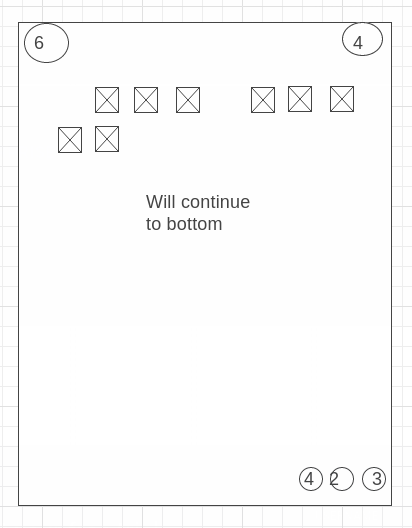
\includegraphics[width=0.6\linewidth]{images/boardWireframe.png}
    \caption{A wireframe created when designing how a board should be displayed to the user. Slots take up the majority of the board, following the design of the physical game while the marbles are collected in the bottom. This is not the final design as an iterative design process was carried during the implementation to improve ease of use.}
    \label{fig:boardWireframe}
\end{figure}

\subsection{Main Page Design}
The main user interface for the plain board was designed after examining other virtual Turing Tumbles as described in the background section. Some design decisions to consider from these programs include
\begin{itemize}
    \item The board should be the largest element and in the centre of the page, giving the most clarity and visual weight to the board.
    \item Piece selection should be on the left and include it's graphical icon.
    \item Options related to the board could be on the left or right of the board.
    \item Triggering the marbles could be placed under the board. To be similar to the flippers in the physical game.
    \item Speed control could be a slider or a list of set speeds.
\end{itemize}

After examining these pages 3 initial wireframes were created for possible page designs. By focusing the design on other implementations it allows users already familiar with these programs to understand this program more easily. The wireframes were created online using draw.io \cite{noauthor_flowchart_nodate}. Different design elements were considered in each with the final wireframe, shown here \ref{fig:wireframe}, being the main design that was improved on during the implementation stage. In this design it was important to have strong emphasis on the board by placing it in the centre of the page with the largest visual footprint. A side navigation bar was chosen to reduce to visual impact of a top navigation bar and was designed to be hidden or reveled by the user with a button toggle when the navigation when required. It was designed that only options available to the user should be shown at any given time and that icons would be greyed out to signify that the option was unavailable leading to less visual weight to useless actions.


\begin{figure}
    \centering
    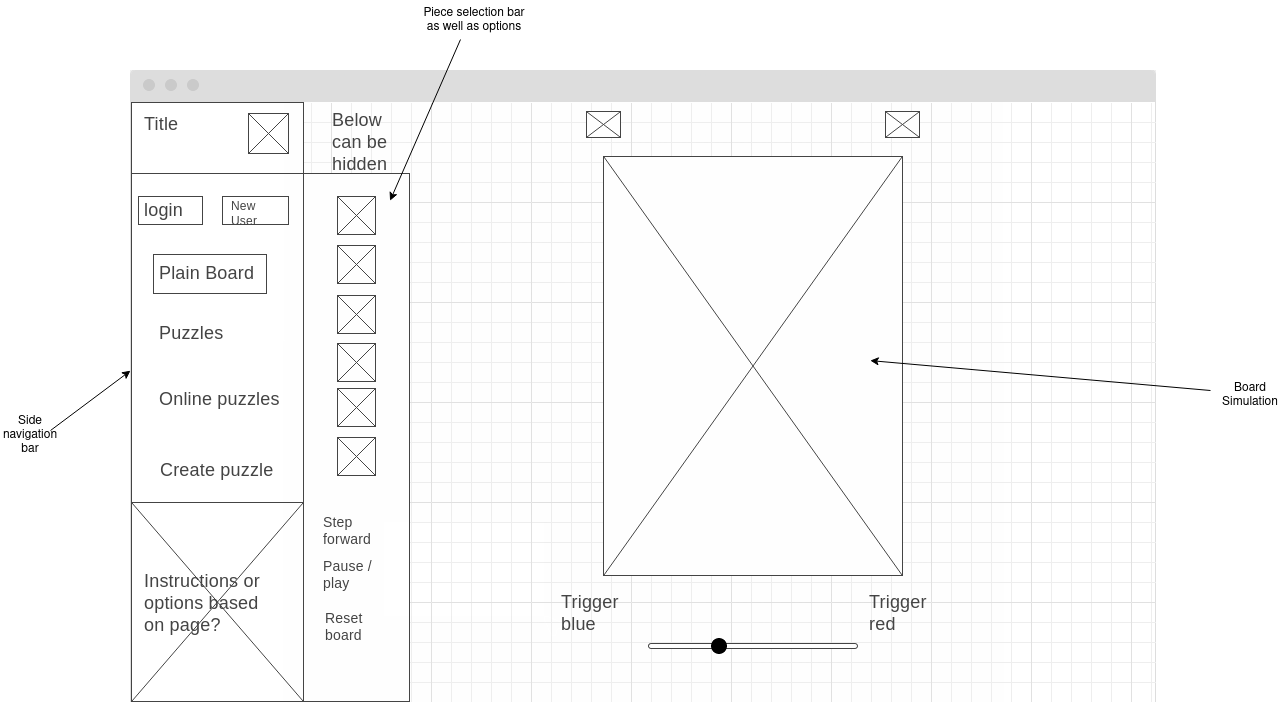
\includegraphics[width=0.7\linewidth]{images/wireframe.png}
    \caption{A wireframe created when designing the main board page. It shows the main position of the board, side selection bar, and side navigation bar with some options. The design changed was revised during implementation and is shown in the implementation section.}
    \label{fig:wireframe}
\end{figure}

\section{Technologies}
The following technologies were chosen to meet the specification and capture the functional requirements.

\subsection{Angular}
Angular (\cite{noauthor_angular_nodate}) was chosen as it is a fully component based Javascript (JS) framework with components split into modules of HTML, Typescript, CSS, and a testing file. Typescript (\cite{noauthor_typed_nodate}) is a super script of JS adding static type checking and allows for greater control over the creation of classes and interfaces compared to standard JS. The components in Angular are organised in a hierarchy and can help keep a strong modular design by passing data down to child components only when necessary. Angular comes prepackaged with some very helpful libraries including a testing framework, routing service, and forms. It is also very easy to add a wide variety of different JS libraries using Node Package Manager (NPM) allowing more development time spent on implementing the functionality of the program instead of solving issues solved by external libraries. While this project is focused mainly with building a web application, Angular can be used to built native mobile applications so the implementation can made more portable as part of possible future work.

\subsection{Material UI}
Material UI (\cite{material}) created by Google was chosen as an external user interface library to add high quality UI elements to the application. Material UI components are highly reliable and already tested to ensure that the UI in the program is easy to use and follows a standard seen in other sites the user may have experience with. Material UI components are added to existing code by using a call to an individual component using Angular notation and editing the component using its API.

\subsection{Web Application}
This program was designed to be built as a web application. One reason was the goal to have this program be easily accessible to the target audience so the high portability of a web application with easy access for many users with a desktop or laptop. Second is that the program was designed with user integration in mind so a web application lends itself naturally to storing user data in a backend server that can then be displayed to other users. Lastly a web application is more accessible for users in a classroom environment, as desktop machines may have different hardware specifications across schools and may not allow external software to be installed easily.


%==================================================================================================================================
\chapter{Implementation}
\section{Angular Framework}
The program was implemented using the Angular framework with Components created to deal with user facing views and Typescript classes created to model the various elements of the Turing Tumble.

\subsection{Angular Components}
Angular components are designed to lead to a natural separation of concerns between it's template, written in HTML, which controls an area of the screen and the application logic contained within it's component class file, written in Typescript. The template file can use two way data binding to interact with it's component class to send and receive data between them, for example displaying data held within the class to the template that can dynamically be updated.


\textbf{Template file}
A component's template file is made up of HTML and Angular template syntax. This file will tell Angular how to render the component to the screen. An advantage of this implementation is it allows the mix of native HTML code and Angular template syntax which can directly edit the Document Object Model (DOM). It also allows calls to child components multiple times with each call creating a new instance of a component with it's own separate data. For example multiple calls to a Component Slot component where each slot has it's own data but they are all created from a single component definition. It also allows for easy creation of a component hierarchy where children components can easily be created and called when necessary as shown in \ref{fig:homeComponent}. 

% Most of the file is written in standard HTML but some important Angular template syntax used in the implementation include
% \begin{itemize}
%     \item \textbf{Angular Directive} - To ensure that templates created by the user are dynamic, angular uses \emph{directives} to transform the template based on the instructions they give. Components are examples of directives as Angular will replace a component selector tag (<app-component>) with the component template at runtime.
%     \item \textbf{<li *ngFor="let item of itemList">} - This is an an example of a \emph{structural Angular directive} which tells angular to repeat the HTML and the children it contains over a list of elements by adding the elements to the DOM multiple times.
%     \item \textbf{<app-example-component>} - This tag links to another user created component, making it a child of the current component. This allows user defined components to be easily mixed in between standard HTML allowing Angular to replace that tag with a call to a component and the template file it contains.
%     \item \textbf{ \{\{componentProperty\}\}} - This \emph{interpolation} syntax allows for data binding between the template file and the component class which contains and can edit the data. If the data were to be updated Angular would refresh the data displayed in the DOM.
%     \item \textbf{[property] = "value"} - This syntax when placed within a HTML or component tag is called \emph{property binding} which can set the data values of child components or set property values in a components API, used extensively for an external component library like material UI. A simple example is <img [src]="imgLink">. The value within the double quotes is a property held within the component class file, named z\emph{imgLink}, this allows the src property of an image tag to be updated dynamically.
%     \item \textbf{<button (click)="clickFunction()">} - The (click) value represents \emph{event binding} in which a DOM event, in this case a button click, can be bound to a response function. In this example a button when clicked by a user will call a \textbf{clickFunction()} held within the component class.
% \end{itemize}

By allowing data binding in native HTML the responsibility of updating data values and ensuring user inputs are captured correctly is given to Angular and focus can be spent on developing the major functionality of the program without spending development time ensuring JS calls are made correctly. 

\textbf{Component file}
The component class file, written in Typescript, contains all the application logic and data related to a view. An example would be a component class for a Turing Tumble piece, which would contain the piece object and functions to deal with a user clicking on a piece. The advantage of these files was that template files could call complex conditional functions which could then be used to determine what data should be displayed in the view.

\subsection{Angular Services}
A service is a class designed for non-UI functionality that can be used by multiple components using \emph{dependency injection} to insert this class into a component at run time. It is Angular practice to design components to only deal with UI logic and leave any functionality related to form input, backend servers, or non-UI functionality in a service which can be called by components when needed. For example a service was created that uploads and retrieves data from a backend server. This allowed one service to be created for this functionality that components could use if they needed backend data without repeating the functionality across multiple components. 


% \begin{figure}
%     \centering
%     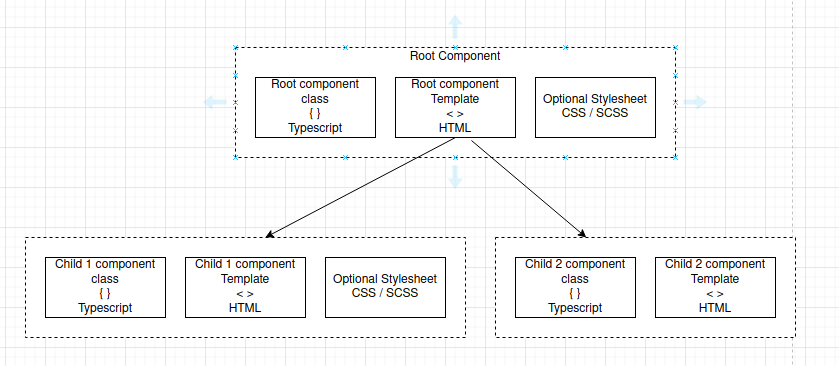
\includegraphics[width=1\linewidth]{images/componentDesign.png}
%     \caption{A diagram showing the files included in each Angular component. Including the hierarchy that is created when calling multiple components Diagram adapted from \cite{noauthor_angular_nodate-1}}
%     \label{fig:angularComp}
% \end{figure}

% \clearpage

\section{Aesthetics}
% \textbf{Material UI} was used to provide a user friendly and visually appealing standard across the program. In which various packages provided by this external library were used including buttons, forms, prompt cards, and side navigation bars. This allowed more development time to be spent on functionality for the program and while some development time was still spent arranging the various UI elements and creating a visually intuitive layout, time was saved by including high quality UI building blocks using this library. It also allowed solutions to common UI problems to be solved by this library, for example the side navigation bar as shown \ref{fig:homepageDark} was implemented using material UI side-nav component module. This allowed for a high standard for user experience across the program without taking large amount of development time.

% \textbf{2 program themes} were created, and a change theme button was added on the heading bar to allow users to switch between a 'dark' and 'light' theme as shown in the appendices \ref{fig:themes}, 'dark' theme is used in all other figures. By having 2 distinct themes it allowed users choose the theme they find the most accessible. The themes are stored in a SCSS file contained at the root of the component hierarchy. This theme change is possible due to material UI and applies to all material UI components, leading to a consistency among all UI elements.
\subsection{Piece aesthetics}
The 6 pieces created for this program were strongly influenced by the design implemented by the physical Turing Tumble board, they can be seen in figure \ref{fig:pieces}. This consistency allows any user familiar with the physical board game to be instantly familiar with the pieces and the logic expected of them. The colours of the pieces were also influenced by the physical pieces and each have a distinct colour separate from any other pieces. This attribute as well as the unique shape of a piece helps improve the recognizability of each piece. Which was found to be no issue in the user evaluation. The pieces icons were created using an online SVG creator \cite{noauthor_method_nodate} and saved as an SVG icon so machines of different resolutions could scale up the icons without losing quality. 

\begin{figure}
    \centering
    \begin{subfigure}[b]{0.20\textwidth}
        
\includegraphics[width=\textwidth]{images/ramp.png}
        \caption{A Ramp piece \\}
        \label{fig:ramp}
    \end{subfigure}
    \begin{subfigure}[b]{0.20\textwidth}
        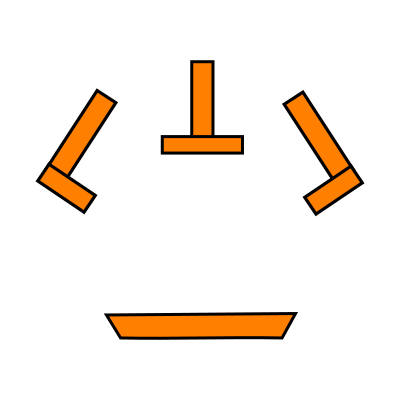
\includegraphics[width=\textwidth]{images/crossover.png}
        \caption{A Crossover piece \\}
        \label{fig:crossover}
    \end{subfigure}
    \begin{subfigure}[b]{0.20\textwidth}
        
\includegraphics[width=\textwidth]{images/bit.png}
        \caption{A Bit piece \\}
        \label{fig:bit}
    \end{subfigure}
    \begin{subfigure}[b]{0.20\textwidth}
        
\includegraphics[width=\textwidth]{images/interceptor.png}
        \caption{An Interceptor piece \\}
        \label{fig:interceptor}
    \end{subfigure}
    \begin{subfigure}[b]{0.20\textwidth}
        
\includegraphics[width=\textwidth]{images/gear.png}
        \caption{A Gear piece \\}
        \label{fig:gear}
    \end{subfigure}
    \begin{subfigure}[b]{0.20\textwidth}
        
\includegraphics[width=\textwidth]{images/gear-bit.png}
        \caption{A Gear Bit piece \\}
        \label{fig:gearbit}
    \end{subfigure}
    % \begin{subfigure}[b]{0.17\textwidth}
    %     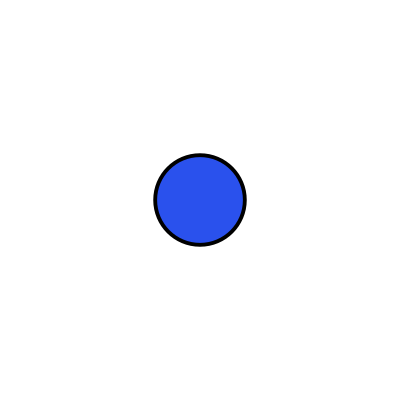
\includegraphics[width=\textwidth]{images/blue-marble.png}
    %     \caption{A blue marble \\}
    %     \label{fig:blueMarble}
    % \end{subfigure}
    % \begin{subfigure}[b]{0.17\textwidth}
    %     
\includegraphics[width=\textwidth]{images/red-marble.png}
    %     \caption{A red marble \\}
    %     \label{fig:redMarble}
    % \end{subfigure}
    \begin{subfigure}[b]{0.20\textwidth}
        
\includegraphics[width=\textwidth]{images/blue-marble-fall.png}
        \caption{A marble falling \\}
        \label{fig:marbleFall}
    \end{subfigure}
    % \begin{subfigure}[b]{0.17\textwidth}
    %     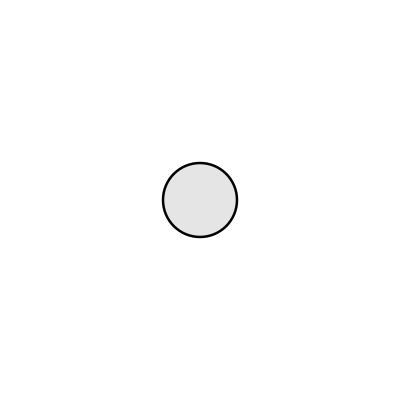
\includegraphics[width=\textwidth]{images/pin.png}
    %     \caption{A Pin}
    %     \label{fig:pin}
    % \end{subfigure}
    % \begin{subfigure}[b]{0.17\textwidth}
    %     
\includegraphics[width=\textwidth]{images/compslot.png}
    %     \caption{A Component Slot \\}
    %     \label{fig:compslot}
    % \end{subfigure}
    \caption{The SVG icons created using \cite{noauthor_method_nodate} for all 6 pieces as well as a marble falling when it reaches no pieces}
    \label{fig:pieces}
\end{figure}

% \subsection{Board aesthetics}
% The aesthetics for the a plain Turing Tumble board as shown in \ref{fig:marbleInPlay} was designed to mimic a physical board as much as possible without adding unnecessary details such as marble dispensers or walls. This minimalist design was chosen to reduce visual clutter and match the design followed by the rest of the program. By having the background a light grey-blue, each piece was designed to contrast with the board background in both themes. The background was also chosen to help give the width and height of the board and ensure that slots didn't appear to 'float'. Two coloured arrows were added at the top of the board to make it easier for users to understand which slot the 2 coloured marbles would enter when first released. The two slot types were chosen to be white to aid contrast with the board background. A blue and red coloured line was added to the bottom of the board to improve understanding of which area are marble would need to be directed towards to trigger the next coloured marble. 


\section{Simulation Features}
This section lists the features implemented to met the main set of functional requirements to have this program match the existing Turing Tumble simulators.
% Each feature should start off at the high level and then more information can be added to describe how it was implemented 
 
\subsection{Board Creation}
Board creation is important to ensure users can create their own complicated Turing Tumble boards to simulate and learn with. Users can select the pieces they wish to place from a selection bar on the side of the page. This selection bar contains the list of pieces including it's graphic icon as shown on the left in \ref{fig:puzzle}, a full page view of the selection bar can be found in appendices. Once a piece has been selected then can place the piece in a valid slot to add this piece to the board. When a user hovers over a slot holding a valid piece, a 'ghost image' is displayed in the slot to give intuition that a piece can be placed, an example can be seen \ref{fig:ghostPiece}. This was a suggestion given by multiple users during the evaluation stage to make it clearer where and how pieces can be placed. Users can delete pieces can selecting the delete piece option and selecting the piece they wish to remove.

Unlike other simulators, users don't need to use a different piece for each direction. Instead if they holding a reversible piece and click on the same type of piece on the board, it will flip it's direction. This was implemented to be more efficient for users to reverse piece direction, this was found to be intuitive in the user evaluations. 

The board component and selection bar were kept separate to improve modularity and single responsibility of classes. When a user clicks a piece on the selection bar this event is captured and sent to the parent component where it then updates the board object. When a user holds a piece, it's corresponding icon on the selection changes colour to aid understanding of which piece is held without an explicit prompt, this is also aided by the ghost image. After clicking a slot on the board, the board will check that a valid slot was clicked before adding this piece to the slot property of the board object. For example users can't place Ramp pieces on Pins, this validity is later extended to capture requirements related to puzzle validity. Within the board component template every slot is created using a separate Slot component that is given it's unique slot contained by the board using an input property which uses Angular data binding to act as a type of parameter for components. This also ensures that when a slot property is updated when a user adds a new piece, the corresponding component updates it's view in the DOM instantly showing this piece to the user in real time.



\begin{figure}
    \centering
    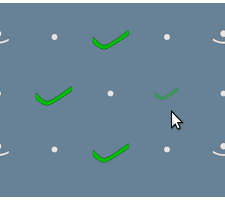
\includegraphics[width=0.4\linewidth]{images/ghostImage.png}
    \caption{A 'ghost image' showing a user where they can place the piece they are holding}
    \label{fig:ghostPiece}
\end{figure}


\subsection{Piece logic}
Each piece available in a physical Turing Tumble board requires it's own logical functionality. To allow every piece to be abstracted in the boards own class implementation, an abstract board piece class was created that contained it's properties including it's type and the logic required to interact with a marble. The logic of every piece was created to exactly follow the logic described in the background section \ref{section:background}. Each piece would be sent a marble to 'process' and would edit it's current direction based on it's properties and call any internal functions required to keep the boards logic. By having each piece represented by class, it allows multiple unique pieces to be created that each have their own state on the board. This is necessary to ensure that pieces placed by users follow the logic found in the physical game while ensuring the board class can leave the pieces state and logic to the individual object.  

% By having each piece extend an abstract class. A single component representing any piece could be created. This component would receive a piece as a parameter and display the necessary graphics to user. By using Angular data binding, this piece would be updated instantly if it's state where to change. For example this would ensure that a Bit piece that had processed a marble, displays this in real time before changing the rotation of it's graphic. By having real time updates of pieces state, it gives users greater understanding of the boards state at any one time.

\subsection{Gear Bit logic}
The most complicated of the Turing Tumble pieces is the combination of Gear Bits and Gears. This combination of pieces is designed to make the board Turing complete and is required to create the most complicated and interesting patterns. Users can connect Gear Bits can placing the Gear piece into Pins separating Gear Bits. Once the Gear Bits have been connected the direction of all Gear Bits are updated to be the same, this ensures that the board enforces the rule found within the physical board. When a user clicks on a Gear Bit to change it's direction, this will also update any connected Gear Bits in it's group. When a marble passes through a Gear Bit, the board will ensure that any connected pieces also change direction.

To reduce the complexity of a Gear Bit's class, the functionality required to simulate this logic was held in the parent board class. When a user places a Gear Bit or a Gear Bit processes a marble an internal function is called to find all neighboring Gear Bits and update their state. This function made use of a breath first style search where Gears acted liked edges between the vertex like Gear Bits. This allowed the Gear Bit pieces to have no knowledge of their sibling pieces and reduce the responsibility of the child Gear Bit class. By pushing this functionality to the parent class, it avoids a complex implementation where each Gear Bit would require the location of any siblings, disrupting the abstraction this class was designed with.

\subsection{Marble simulation}
A user must be able to simulate the path a marble would take following the selection of pieces on the board. This is required for a user to understand the effect the displayed pattern of pieces would have on the marble. After placing valid pieces onto the board, a button can be clicked to release a red or blue marble. The marble will be released at the top of the board and will then move down having it's direction changed by interacting with the pieces. If a a marble reaches a empty slot, a 'falling' icon \ref{fig:marbleFall} is displayed to indicate the marble has been reset. This ensures that a user is given feedback to why a marble path was not valid. Each piece has an icon of a marble interacting with the piece, this was created to give the illusion of the marble falling through each piece while ensuring the marbles position is always displayed the user.

The marble in play has it's on state which is updated by each piece it visits. The marble is held by the board object and ensures new marbles are released when it reaches the end of a valid path. By keeping the marble class simple, it allowed for an easier implementation of marble simulation by leaving the responsibility to the parent board class which can update and remove marbles when required. 

% Marble validity is achieved by the design of the Turing Tumble board. Pieces can only send marbles to another Component Slot so will always follow a valid set of pieces if present. The walls of a Turing Tumble were implemented by constraining a marbles position if it is sent outside the board width, this allows the fallen marble to appear before it is reset. Ensuring a marbles position is always visible to a user when in execution.

% Two marble dispenser components were created to be displayed above the board. These components had the logic responsible for displaying the amount of marbles available to be released onto the board, it also included 2 buttons to increase or decrease the amount of marbles available. 
To reduce the space required by captured marbles which caused issues in other implementations. A collected marbles class was created that only stored the coloured marble sequence collected by a board. This can be seen at the bottom of \ref{fig:marbleInPlay} in which 5 collected marbles are only represented by 3 icons to reduce visual clutter displayed to the user.
   
\begin{figure}
    \centering
    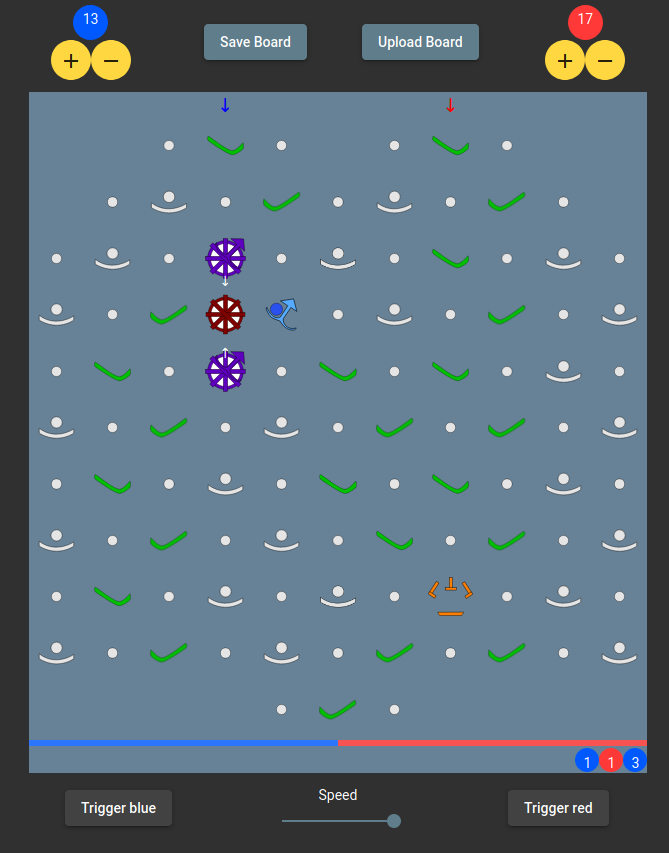
\includegraphics[width=0.5\linewidth]{images/marbleInPlay.png}
    \caption{A view of the board while a marble is currently in play and is displayed to the user. Collected marbles can also be seen at the bottom section of the board}
    \label{fig:marbleInPlay}
\end{figure}

\subsection{Playback features}
An important requirement of the program was to provide execution control to aid in user's understanding of the boards execution. A function was created to implement a single iteration of the marble travelling down the board. Playback functions were then implemented that dealt with calling this function in different sleep intervals to mimic the physical time required by a marble to travel. A pause / play feature was added to allow users to pause execution when required to better understand the path the marble is to take. A speed slider was added below the board to allow users to change the amount of time the execution loop would wait. A slider was added for more accurate execution control compared to a list of presets as found in other implementations. A step forward function was implemented that allows user to click a button to pause the current execution and jump to the next location without waiting, this can be clicked based on the users desired stepping speed and allows stepping past more simple piece patterns or stepping slowly through more complicated logical components without needing to pause and play. 

\subsection{Board options}
4 separate options were added to aid user control over the board. A user can reset the board removing all placed pieces while deleting the collected and in play marbles. This gives the user a quick reset function without requiring excessive time spent deleting the individual pieces. A similar reset marbles option was also added to allow users to remove the in play marbles and any marbles collected, useful to slightly edit the pattern on the board while resetting the output.

4 example boards were created from inspiration from JSTumble (\cite{jstumble}) and the Turing Tumble home page. These examples can be accessed by a button press on the plain board page. It will add the selected piece layout to the board and allows the user to work through more complicated examples of the computational powers of the Turing Tumble. This was added to improve users awareness to the computational capabilities of the Turing Tumble without requiring them to create the patterns from scratch. 

\subsection{Save and upload Patterns}
A save and upload board feature was implemented following the design discussed in section \ref{section:design}. Functions were created to convert an array of slots into a string and vice versa. The implementation allows for an efficient way to represent and store a boards patten that users can then easily understand and edit outwith the site. The functionality is stored in an external class so it can be used by both components and services requiring the convert functions.

\section{Puzzle Features}
The most important features implemented in this program was the addition of puzzles. Allowing users to play through the set of default Turing Tumble puzzles found in the educator guide (\cite{educator_resources}) directly within the program, gives users a fun external motivator to play and learn with the simulation. Puzzle creation was also implemented to allow for the creation of a puzzle ecosystem in which users can create new puzzles for others to play, directly increasing the enjoyment users can have on the site as well as the possible learning effects the puzzles can have.

\subsection{Puzzle List}
A user can find puzzles from two pages. 'Original Puzzles' which will list the puzzles created from the puzzles provided in the Turing Tumble educator guide, and 'Online Puzzles' which will list the puzzles created by other users of the site.

For each page, a list of puzzle card components is given on the screen. The list of puzzles has been limited to 10 cards per page, with a paginator added to the bottom, where users can move through the list of puzzles available. Each puzzle card component as shown in \ref{fig:puzzleList} lists the 6 descriptive properties used in determining what the puzzle entails. 
\begin{itemize}
    \item Title - The name given to the puzzle
    \item Description - The description of a puzzle contains a one or two line summary as to the purpose of the puzzle and what a user should expect to achieve or learn.
    \item Difficulty Rating - The difficulty rating of a puzzle is used to categorize the puzzles into 5 distinct groups based on a 5 star difficulty scale. This scale was chosen to mimic the scale found in the physical Turing Tumble to allow a direct relation between puzzles created for the physical game and any user created puzzles.
    \item Starting Set up - The starting set up attribute displays a board with the starting pieces which cannot be replaced or deleted by the user. These pieces constrain the puzzle and the way the user must meet the expected output.
    \item List of Pieces available - The challenge of the Turing Tumble puzzles come with the restriction of pieces available to reach the expected output of the puzzle. This restriction ensures users follow a set pattern of computation to meet the expected output and can create a variety of different challenging puzzles even if they share the same expected output.
    \item Expected output - This lists the collected marble output that the board should receive to complete the puzzle.
\end{itemize}

A difficulty filter has been implemented allowing users to filter the list of puzzles shown by the set of difficulties they wish to view. This gives the users greater control as to which puzzles they wish to view without having to  go through multiple pages of puzzles that may not interest them. This filter was also implemented to help organise the list of user created puzzles. A clear difficulty progression is present with the default puzzles but with online puzzles it currently lists any puzzles created by users based on the time created so by adding a filter users can ensure they only see puzzles of interest. The filter updates the list instantly and doesn't require the page to be reloaded when a new set of difficulties is selected, this adds to usability and avoids unnecessary load times for users.


\textbf{MAYBE ADD TO DESIGN SECTION INSTEAD?}
% The list using a material UI expansion panel to only show the title and difficulty of a puzzle until a user clicks the puzzle bar. Upon clicking, the user is given a set of tabs they can use to view more information about the puzzle, including it's starting set up and list of pieces available. This expanded view also gives the user a button to launch the puzzle. This ensures the list is clean and compact until the user clicks a puzzle they are interested in.  

\begin{figure}
    \centering
    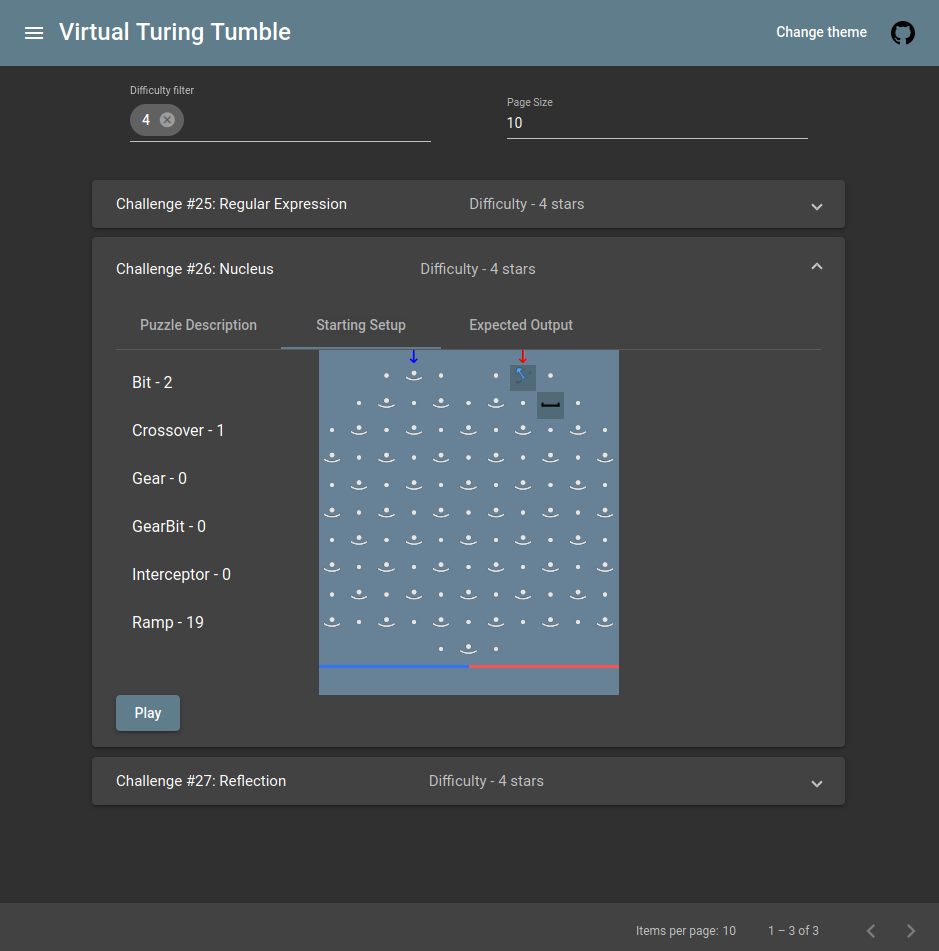
\includegraphics[width=0.65\linewidth]{images/puzzleList.png}
    \caption{A view of the puzzle list used in both the original puzzles and online puzzle pages. One puzzle card has been expanded after clicking, displaying more information about the puzzle}
    \label{fig:puzzleList}
\end{figure}

\subsection{Playing a Puzzle}
A user is presented a board view which uses the same component found in other parts of the program. The user is also given a puzzle title and description above the board to ensure the user understands the puzzle's objective. An example of playing a puzzle is shown in \ref{fig:puzzle}

A puzzle also limits the number of pieces available to a user to place on the board. This is given by a number next to the pieces icon on the selection bar component. This number is updated dynamically when user's place and delete pieces on the board. The button to select a piece is disabled when the user has no pieces to place. This ensures users understand the exact pieces available to them to complete the puzzle, adding to the learning and challenge of the objective. 

The starting pieces are highlighted with a darker background compared to the normal slots. These are seen as 'locked' and users can't edit the pieces held within these slots. This background change was added to helped distinguish these slots from the pieces users can place.

% The normal marble buttons used to increase the number of marbles available have been removed as the number of marbles available to complete the puzzle are set as part of the challenge. This ensures the users understand the options aren't available.

A next puzzle button has been added above the selection bar as suggested by a user during evaluations. This will start the next puzzle by updating the data in the component without requiring a reload from the user. The next puzzle is taken from the list that has been filtered by the user, ensuring they only play the next puzzle they are interested in.

\begin{figure}
    \centering
    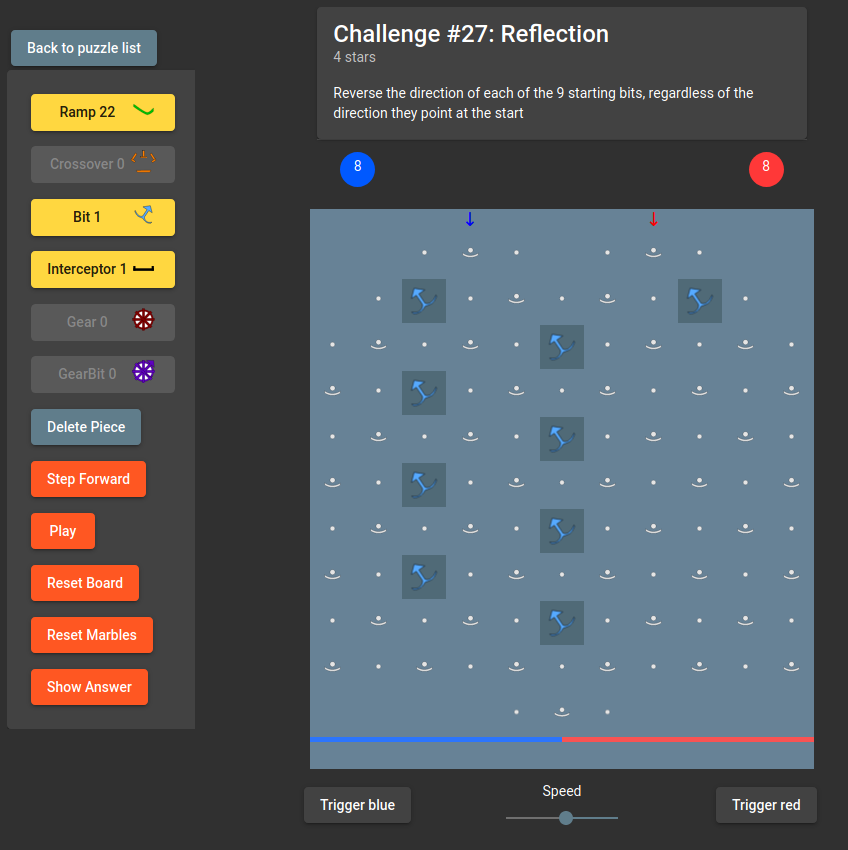
\includegraphics[width=0.65\linewidth]{images/puzzle.png}
    \caption{The view displayed when playing through a puzzle, including the number of pieces available to a user in the selection bar}
    \label{fig:puzzle}
\end{figure}

\subsection{Puzzle Class}
To implement and store details of puzzles, a new Puzzle Board class was created which extends the existing board class used to represent a normal Turing Tumble board. This extension allowed all functionality used in simulating, placing, and deleting pieces to be reused by users when playing a puzzle. By reusing the functionality found in other sections of the site, code duplication is avoided and the user can use the knowledge learned by using the plain board to play through a puzzle. Major extensions of functionality include the puzzle board using the board class' piece placement functionality and checking if a slot had been changed using this function. It could then use this to determine if the piece placement by the user was successful, then updating any piece constraints required by the puzzle. By reusing this functionality, any changes to how users could place pieces will automatically be available for puzzles as well. This was useful for the possibility of future work if a drag and drop feature were to be implemented. 
% Another important piece of functionality that had to be replaced was the reset board option. In the puzzle implementation it was required that resetting the board didn't break the piece amount constraints so the amount of pieces available to the user had to correctly reset.  

% \textbf{Puzzle validity}
% It was important to ensure any user playing the puzzle couldn't cheat their way to the congratulations message. While the completion of a puzzle is only for self satisfaction, future work can be dedicated to adding leaderboards or user statistics detailing the number of puzzles users correctly solve. This requires a strong set of functions that ensure completion of a puzzle by a user is from their own merit and not by cheating. 

% This was ensured by not allowing extra marbles on the board to be added or removed by the user, so a single execution of the puzzle would be all that would be required to reach the expected output. A user can only reset the board's available marbles by using the reset marbles function which also removes the marbles collected by the board. This ensures users can't send down one marble correctly, reset the marbles and send down the next correct colored marble.

% The amount of pieces users have to complete the puzzle is enforced and checked before a piece can be placed, this ensures no puzzles can be completed outwith the puzzle constraints. 

% \subsection{Puzzle Component}
% The puzzle playing component reuses components already created for other parts of the site. This ensures internal consistency between the different sections of the app. For example the selection bar component is used in multiple pages that allows placement of pieces on the board is present here with different parameters given to this component as part of it's created API. This allows the selection bar to update the options and piece information it displays while keeping the same structure and view between two separate pages. 

% The puzzle playing component also makes use of a prompt card component which uses data interpolation to display the different puzzle attributes in the same format for any puzzle that is played. This abstraction is handled by Angular and allows heavy reuse of this component.

\subsection{Creating puzzles}
A puzzle creation system was implemented to met one of the major goals of the project. The creation of a puzzle was implemented using a phase system where underlying functions would have different logic depending on the phase a user was in. 

Puzzle creation was implemented using the existing board functionality. This allowed for efficient code reuse but also ensured that the users would already be familiar with how to place and create a pattern on a Turing board so reduced the barrier of entry for a user to create puzzles.

An authentication system was added were users could login to the site either anonymously or using Google login. This would allow puzzles created by using to have the authors name. This feature was added when a User page was still a main requirement however due to time constraints this was reduced in importance. However authentication is present to ease implementation of any future work requiring it.

\textbf{First phase}
The first phase a user would enter the page in was the starting set up phase. This asks the user to place the pieces that will act as the starting set up for a puzzle. Users only have the option to place the pieces needed for a starting set up, and other unavailable options have been hidden to ensure the user isn't given distracting visual clutter. The user is given details of what is expected of them in a prompt component at the top of the board. After placing the starting pieces, a button can be clicked to confirm the set up. 

\textbf{Second phase}
Once the puzzle's starting slots have been confirmed the user is asked to places the pieces required to solve the puzzle. When placing pieces, the selection bar will take note of how many pieces have been placed in this phase. This will store the amount of pieces a user will have when they play the puzzle. A user can solve the puzzle in fewer pieces but the solution created by the author is the least efficient solution possible. Once the solution pieces have been placed a user can  add the marbles required and then execute the board using the triggers familiar from the plain board. Once the collected marbles matches the target result the user clicks a button to confirm the board set up and output. The second phase is shown in \ref{fig:puzzleCreation}. At any time a user can return to the previous set up if they made an error. This was a suggestion given by a user during evaluations to improve the puzzle creation process.


\begin{figure}
    \centering
    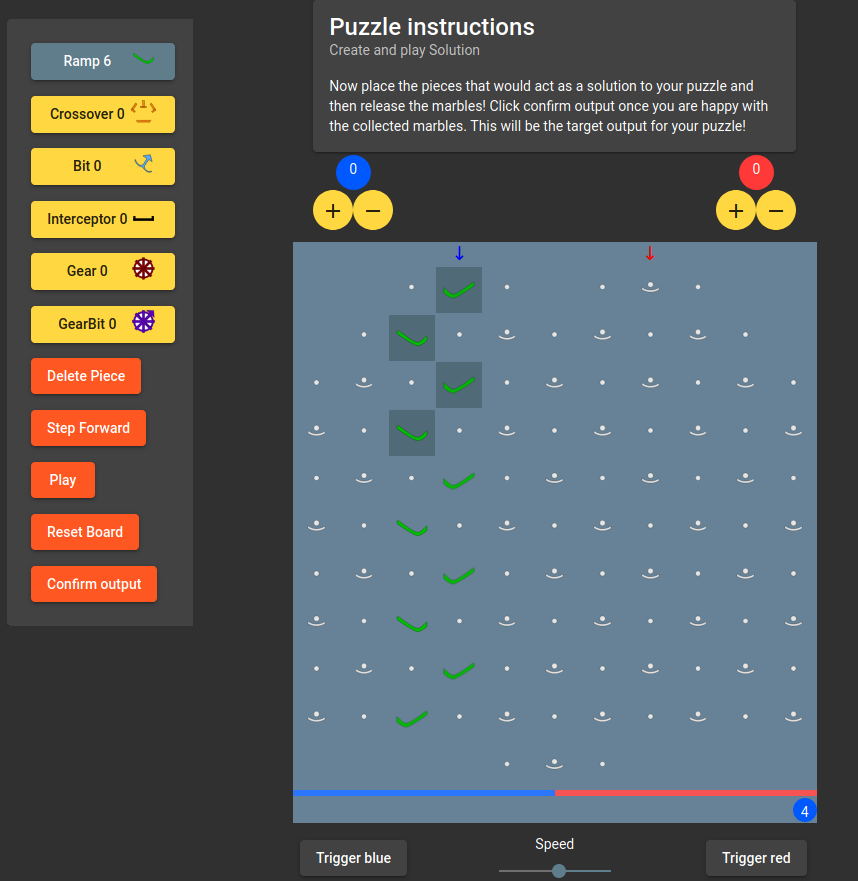
\includegraphics[width=0.65\linewidth]{images/puzzleCreation.png}
    \caption{The second phase of puzzle creation where users must adding the pieces needed to create a solution to the puzzle}
    \label{fig:puzzleCreation}
\end{figure}

\textbf{Final phase}
The final phase gives the user a simple form to input the title, description and difficulty attributes for this puzzle. After ensuring this values are valid the puzzle is then submitted by a user click.

\subsection{Puzzle Creation Functionality}
The underlying functionality uses a combination of the puzzle board class, a puzzle object, and an external service containing the backend functionality. The puzzle class uses functionality extended from the base Board class but holds a property related to the phase a user is in. Depending on the phase, different functions will store values related to the puzzle, including the starting pieces on the board and the number of pieces required for a solution. After confirming the puzzle output, the external service is used to upload the board to the backend Firebase (\cite{firebase}) server.

\subsection{Puzzle Creation Validity}
To ensure a user creates a puzzle which is possible to be solved correctly by an anther user. Validity was implemented in the functions users used to create the puzzle based on the design described in \ref{section:design}.

To ensure the correct starting pieces are identified, a user must set the starting slots first before moving onto the solution creation phase. These slots are saved so can be retrieved when playing the puzzle.

The number of pieces available to a player is not set as input by the puzzle creator. It is calculated during the creation phase where a creator places the pieces required for a working solution to the puzzle. This ensures a user can not create an impossible solution to solve.

The amount of marbles available to a user is calculated by increasing a property whenever a creator increases of decreases the amount of marbles available. This again ensures that a user can not create and upload a puzzle that is impossible for a user to complete. 

By enforces the expected output of a puzzle to be confirmed by a user playing through their puzzle. This ensures that the puzzle created is feasible and can be completed by at least one user, the creator. This was implemented instead of a possible creation form where users could could create puzzles that were either impossible or harder than the creator could solve.

By implementing built in validity through the creation phase, any puzzles uploaded to the backend server are by design valid and solvable. This is important to future work where more emphasis can be added on nurturing a puzzle ecosystem for a large number of users. It also adds to user enjoyment by ensuring that a user couldn't play a broken puzzle in the online puzzle list.

% \textbf{Puzzle Creation Component}
% The puzzle creation page makes use of the selection bar, board component, and a information card. The selection bar is given input for the puzzle that is being created and as the current creation phase changes with the user creating the puzzle. The selection bar updates which options it will show or hide to the user. The board component works identically to other parts of the site, but ensures that the users starting set up pieces update to the their locked state once confirmed. A information card component is added to the top of the page to give the user more information on the stages of the puzzle information. This was to give easier instructions to a creator without requiring them to reread the tutorial. 

% The final phase puzzle creation uses a simple material UI form view. Giving the user text fields for text and description, as well as a 5 point ratio box list to enforce difficulty is constrained without the range. The form fields are stored in the external service and enforce all fields are filled before submission.

\section{Usability}
A key goal of the program was to ensure high ease of use and clear for all users but especially users unfamiliar with a Turing Tumble. 

\subsection{Home page}
A home page was created to give users an access point to enter the program that gives details about the program, including why it was created, a section detailing the tutorial page, and a brief description about the Turing Tumble board with a link to it's website. It was important that users had a clear understanding of what the program was about as well as giving them direction to the tutorial page in which they can learn more about how the program and the Turing Tumble. The section on the Turing Tumble is designed to get users interested in the Turing Tumble, providing motivation to use the site. The home page also includes 4 boards at the bottom representing the example boards users can open in the main board page. This gives users some examples of how the board is represented on this program and shows them more complicated patterns to capture interest in the board. The home page can be seen in \ref{fig:homePage}.

\begin{figure}
    \centering
    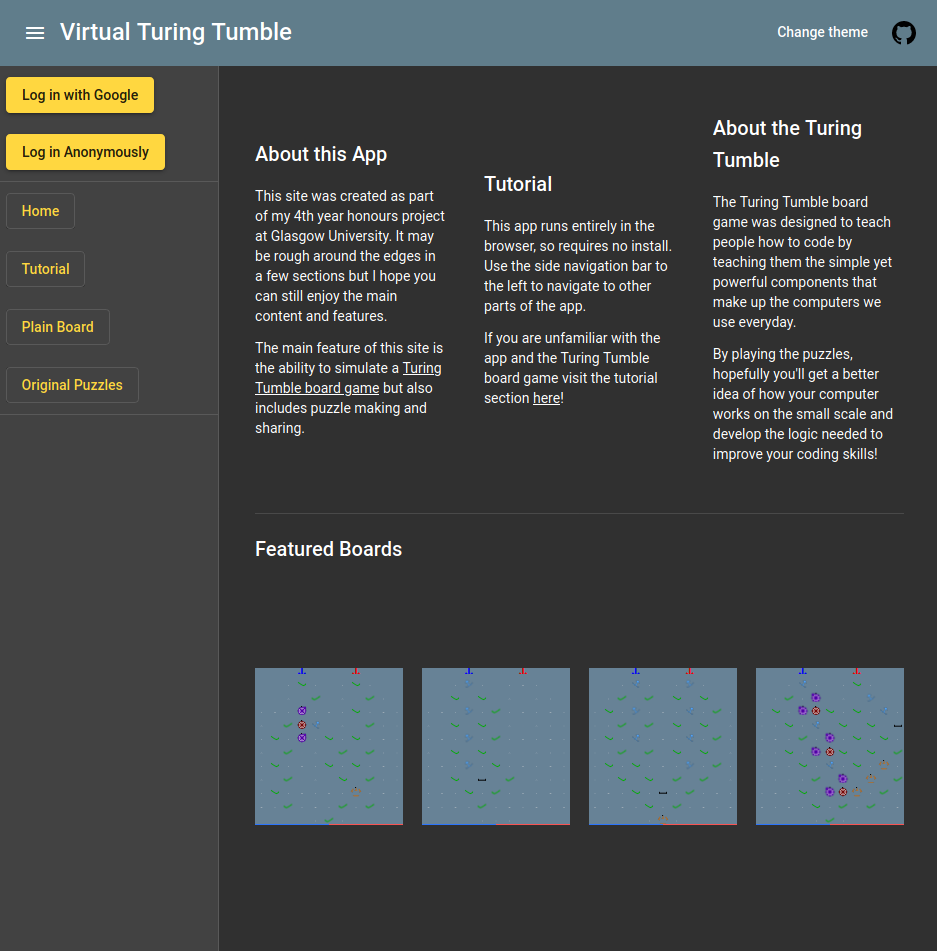
\includegraphics[width=0.65\linewidth]{images/darkTheme.png}
    \caption{A view of the home page of the program, with three paragraphs detailing what the site is about, the tutorial page, and what the Turing Tumble is.}
    \label{fig:homePage}
\end{figure}

\subsection{Tutorial}
A tutorial page was created to give users information on different parts of the program. Three sections were created detailing the following information.
\begin{itemize}
    \item Lists information about each page in the program and how to reach these pages using the side navigation bar.
    \item Gives a brief description into the concepts and gameplay of a Turing Tumble and how it is represented in the program.
    \item A description of the options available when simulating a board.
    \item A table detailing the name, image, description, and what every piece is metaphorically like. This helps users get all the information they need to use the pieces.
    \item Details how to access, choose, and play a puzzle.
    \item Underlines the three phases needed for a user to create their own Turing Tumble puzzle.
\end{itemize}

It was important to include a page with detailed instructional information so users would have an understanding of how a Turing Tumble works and how it is simulated in this program. The main target audience of the program are users unfamiliar with the Turing Tumble so a brief description of the game was required to give context to the simulation. Detailed information is available on how each individual piece works to ensure users understand why each piece is useful in the context of the game. This can be seen in \ref{fig:tutorial}

\begin{figure}
    \centering
    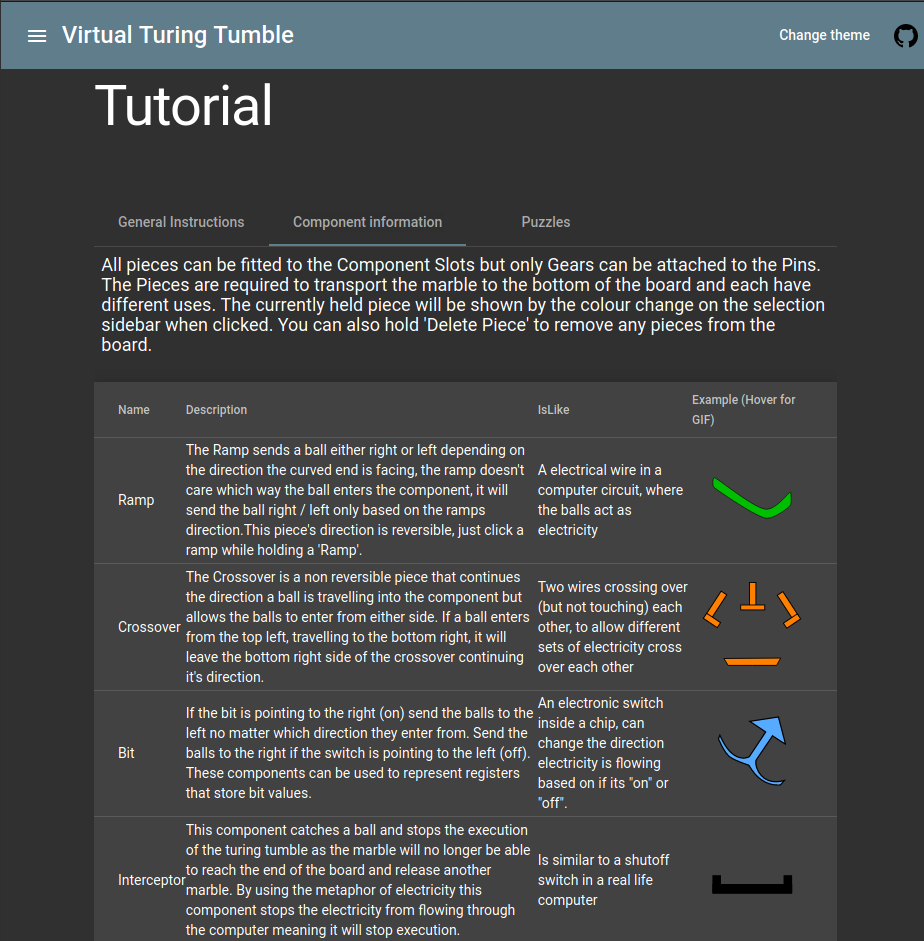
\includegraphics[width=0.65\linewidth]{images/tutorial.png}
    \caption{A view of the tutorial page of the site, including the three separate tabs users can use to access different information sections.}
    \label{fig:tutorial}
\end{figure}


\section{Backend Service}
A service was created containing the relevant functionality to upload and download data from the backend Firebase server. The Firebase server was easy to use and required simple API calls to interact with the server. This approach was taken to minimize time needed to be spent on a backend implementation, focusing instead of the puzzle features for the users. 

This service is injected into the different components. The puzzle creation component uses this service to set and then upload the puzzle created by the user. The puzzle list component, used by both the default puzzles and online puzzles, uses this service to download the specific list of puzzles stored. By injecting this service in multiple components, functionality is reused when required, instead of explicitly rewriting this functionality within components requiring it.

When uploading a puzzle, the details of a puzzle are converted into a smaller more data efficient object. The starting and solution slots for a puzzle board are converted into their string representations using the functionality present used downloading boards. The puzzle is then converted into JSON and uploaded as a string. This allowed for simple upload of the exact puzzle details to the server while maintaining a small file size. It was important to optimise the size of the puzzle upload to ensure that download times for users remains small. By keeping download times small, the user experience will be improved when viewing the list of puzzles. When a call is made to the server to upload a list of puzzles, the JSON representation stores the data of the objects but discards all type information when uploading. A converter function was created as described in section \ref{section:issues}. This function is used to convert a board represented by a string into the correct types.

The form used to add puzzle details is also stored within the service. It ensures that all entered by the user is required and a difficulty validator was created to ensure no values outwith the range could be entered. 

\section{Component Implementation}
Angular encourages a component approach when developing. This design principle was followed as much as possible when creating abstract and interactive components. By focusing on creating small compact components, many pages would utilise a set list of components already used in different sections of the page. As shown by the component diagram \ref{fig:homeComponent} for the Home page. The same board component is created 4 times each with it's own individual list of slots and pieces. This allowed all components to follow one source of truth and lead to high reuse of existing code. 

An Input tag can be added to any property in a component class to allow this property to have a value passed to it as parameter, this is called \emph{property binding}. This allowed components to abstract exact details of what data they were displaying to users and allow components to be created for interfaces or abstract classes. One example were this was used heavily was the piece component. A BoardPiece property that could be bound by a parent component allowed for any of the six components to be passed and utilized in this component class. Ensuring that a consistent design and reuse of code was implemented for all 6 pieces. 

An output property can be added to a component allow data to be sent 'up' to the parent component by creating an event emitter. The parent component can then capture this event sent by the child component and call a function to deal with the event. This is used heavily in the selection bar component which contains output properties to signify when a button is pressed by the user, the parent component will then capture this event and update the board. This allowed the selection component to not have direct access to the board object and not been given details on the implementation of the options it presents to the user. 

As each created component holds it's own independent data, multiple components can be created without data being shared. This is most useful when creating the slots on the board object. Over 106 separate slot components are created to handle the data and any user events for each individual slot. This allowed the functionality for a single slot to be implemented then repeated for each slot on the board.

\begin{figure}
    \centering
    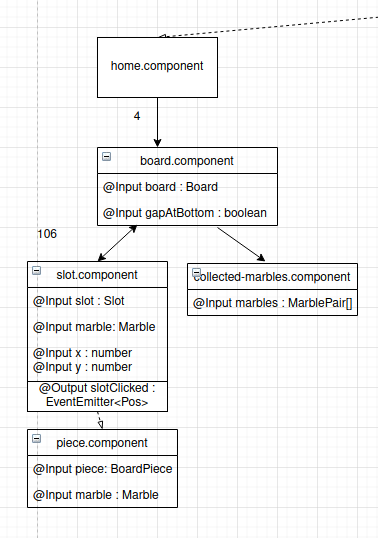
\includegraphics[width=0.45\linewidth]{images/homeComponent.png}
    \caption{A view component hierarchy including the number of child components this page reuses.}
    \label{fig:homeComponent}
\end{figure}

\section{Deployment}
The site was deployed using Github pages (\cite{soloproject}). This allowed easy deployment to a free and always online platform. It was decided that the site would be deployed to ensure that the target audiences of the program can access the program without downloading or installing the necessary files or libraries required to run this program on their own computer. 

\section{Documentation}
Documentation has been created to provide guides to other developers on how to install and run this program on their machine. Extensive code documentation was created detailing ever major class and component. This documentation will help other future developers edit and add new features to the program, improving the overall maintainability.


\section{Issues experienced during implementation}
\subsection{Passing Router parameters}
\label{section:issues}
Routing between different views in Angular, is implemented via a 'Router Outlet' component. This component is placed at the root of the web page and then a 'Router Link' can be created between a URL and a component to display. Originally the 'Original Puzzles' and 'Online Puzzles' pages used the same component but depending on the link clicked by the user a puzzle destination was passed as a parameter to obtain the specific list of puzzles. This allowed a link to 'Original Puzzles' to access a generic puzzle list component while passing the path to this list of default created puzzles. The same would have been repeated for Online Puzzles, however when passing this parameter to the router it would display the correct list initially, but if a user was to navigate from 'Original puzzles' to 'Online puzzles' the Router Outlet would not detect a change of component, so would therefore not call the component creation function which pulled the exact data from the Firebase server, leading to no change in view for the user. This was fixed by creating 2 separate components for 'Original Puzzles' and 'Online Puzzles' that had a child component of the abstracted puzzle list component passing the list path using property binding. This allowed an abstract component to be used for both lists of puzzles while ensuring all routing to these components worked as expected.  

\subsection{Converting data pulled from backend server}

The program was designed with a focus on an Object Oriented (OO) approach, we decided to have Typescipt classes to represent the various objects used in the program, for example a Board and Ramp class. This allowed development to focus on keeping data and methods contained within the objects requiring them. This allowed a separation of concerns between each individual class and reduced the reliance on external services to update board state as originally designed. One issue arose when uploading puzzle data to the firebase server. The data stored in the Firebase server would lose it's type information. This caused puzzles downloaded to not correctly execute as the data held had no references to the class methods required to update state. 

To ensure that data downloaded from the server contained the correct type data, a converter function was created within the external 'make puzzle' service. This converter function would loop through all properties of the data downloaded and assign each property to a new instance of the object required. This fix allowed puzzles uploaded to be downloaded with no data or type loss. Future work can be spent making this function more efficient which would reduce load times for users.

\subsection{New GearBit when turned}
The most complex and interesting piece in the Turing Tumble is the Gear Bit and the relationship they have with Gears. The original implementation of this feature had the GearBit object calling a function in an external board service which would check if it needed to change it's direction by inspecting the state of the board and if the piece was connected to any other Gear Bits. This implementation bypassed the Angular component child relationship and caused warnings to appear and Gear Bits to render incorrectly. This was because a board component would finish rendering to the screen and then a child component would then edit it's view bypassing the parent. This goes against Angular best practice so a new implementation had to be designed. Refactoring was undertaking and the functionality required to move sets of Gear Bits was moved to the board object instead of being in the individual GearBit objects. This allowed the view hierarchy to be preserved as the board component contains a board object which would edit it's Gear Bit child. This ensured that the child component's data, the Gear Bit, was only edited by the parent so could be rendered in teh correct order by the Angular framework. 

% \subsection{Sets not checking objects}
% For the implementation of GearBit functionality, a breadth first style search function was created to discover the set of all Gear Bits connected via Gear objects. The function required a set of visited Gear and GearBits. An issue was found using the built in Javascript (JS) Set object. The project was written in Typescript, the superset of JS that adds type checking and custom classes. Custom class was created to store the position of each visited Gear or Gear Bit. It was then discovered that the set object in JS doesn't contain type information so any position object added to this set was unique, even if two position objects contained the same x and y property. This lead to issues when clicking a GearBit as it wouldn't exit the loop trying to find all connected pieces, as the base case would never be met, so would search infinitely.  To fix this issue a built in library was used to convert this position object into a string JSON representation, this could then be stored in the set as expected for the breadth first algorithm. 


%==================================================================================================================================
\chapter{Evaluation}

Evaluation was carried to out to analyse if the program meets the functional and non-functional requirements discussed in the design section. Unit tests were created to ensure functional requirements of the program were meet. Angular end to end tests were made to test UI functionality while user evaluations were carried out to gain suggestions for improvements and feedback on ease of use of the application. Some suggestions have been added to the future work section while others are just discussed. 

\section{Unit Testing}
Unit tests were created with the Jasmine testing framework which came packaged with the Angular project. These tests were created to ensure that underlying code met the functional requirements and simulated the logic of the Turing Tumble as expected. These tests were also created to ensure that any refactoring undertaken had a safety net to ensure that no internal functionality was accidentally changed. Test coverage was calculated using the testing framework and is shown in the diagram \ref{fig:codeCoverage}. 

The diagram shows the statistics of the testing coverage provided by the unit tests. Classes were given the most comprehensive tests as they focused more on the underlying logic of the program and included aspects of the program that should never change, for example the logic of the pieces should always reflect the logic found in the physical Turing Tumble game. The test coverage for components was lower as the tests created did not cover all the UI elements that are displayed in the components HTML file. This was seen as acceptable as focus was given to testing the functionality for the program and less so on visual elements that would be displayed. In hindsight given the importance of creating an application that is visually appealing to users, more tests could have been created to ensure logic related to UI was under test. An overall statement coverage of 73\% was achieved showing that most aspects of the program were inspected and tested for correct functionality.

Important Unit tests that were created include
\begin{itemize}
    \item Connected GearBit components will have the same direction and all change when one is clicked.
    \item A user should be able to select a piece from the sidebar and then place this piece in a slot.
    \item The board should allow a marble to reach the bottom and then trigger the next coloured marble corresponding to the location that it lands in.
    \item When a new GearBit is connected to a set of GearBits it should change it's direction if required to ensure the set of GearBits all face the same direction.
    \item GearBits should marbles in the opposite direction to where they are facing and then should switch direction.
    \item Ramp pieces should send marbles in the direction they are facing.
    \item Crossover pieces should send marbles in the direction they are currently travelling.
    \item Bits should send marbles in the opposite direction to where they face, then change their direction.
    \item Interceptors should stop the marble travelling.
    \item PuzzleBoards should lock the starting pieces of a created puzzle when confirmed.
    \item The amount of marbles in a puzzle should only be increased if in the creation phase.
    \item Puzzles should update the number of pieces available correctly.
\end{itemize}


\begin{figure}
    \centering
    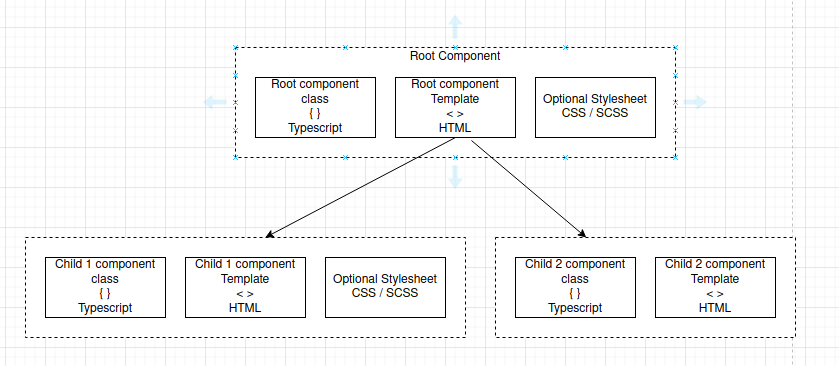
\includegraphics[width=1\linewidth]{images/codeCoverage.png}
    
    \caption{This code coverage table was produced by the testing framework and shows the test coverage for different parts of the program including the typescript classes and Angular components created.}
    
    % use the notation fig:name to cross reference a figure
    \label{fig:codeCoverage}
\end{figure}

\section{UI Testing}
UI tests were created using the built in end to end testing framework 'Protractor'. This framework would allow certain DOM elements to be checked if visible and could allow simple button presses and router navigation. These tests would launch an instance of the site and travel through various pages by mimicking button presses. 

These tests ensured that the elements were still displayed correctly even when underlying component logic was changed or updated for example tutorial page information was still visible after adding a ta system. The tests were black box in style and didn't test underlying functionality only that the correct content was displayed to the user and that the user could navigate to the various pages. 

Test covered include 
\begin{itemize}
    \item A welcome message should be displayed to the user on the Home page.
    \item The side navigation bar should be opened and closed by the hamburger icon.
    \item A user should be able to select a piece to place on the board.
    \item The user should be able to navigate to the Tutorial page.
    \item The three separate tutorial sub sections should be visible.
    \item The theme of the program should be changeable by the user.
    \item A set of puzzles should be viewable when navigating to the Original Puzzles page.
\end{itemize}

\section{Monitored User Tests}
Monitored user tests were carried to ensure that users could complete the tasks while having the option to ask for help or explanation if the tasks or site wasn't clear enough to use. The users were encouraged to give suggestions and improvements while working through the tasks and these were recorded. This allowed the user to give feedback on any aspect of the site, including aspects that were omitted from the evaluation form. 5 4th year Computer Science students were chosen for this test, this meant they should find the Turing Tumble game intuitive so would be able to focus on the websites ease of use instead of the games logic. The meetings were recorded so points made by the users can be recovered at a later date. The task sheet given to the users included 4 tasks and did not included a lot of detail or explanation of how to complete the tasks, for example they were asked to input a pattern without instruction to using the selection bar. This allowed for analysis to focus mainly on the ease of use that a user would have if they were to access the site separately and only have the tutorial to explain it's functionality. The tests took place over Zoom and the notes from these meetings can be found in the appendices.

\subsection{Task Explanation}
\label{taskExplanation}
Users were given an initial set up task followed by 4 tasks, one of which was optional

\begin{itemize}
    \item \emph{Task 0} - Asked the users the navigate to the tutorial page and spend some time reading the page giving basic details of the Turing Tumble game plus the functionality of the site.
    \item \emph{Task 1} - Asked the user to navigate to the plain board and add pieces to the board and walk through a basic Ramp pattern. They were then asked to experiment with the Bit and GearBit pieces. This allowed users to experience placing pieces and playing a Turing Tumble board. It also gave an opportunity to give the user an experience with the two of the more complicated pieces and focus on why they are important for the boards possible complexity.
    \item \emph{Task 2} - Asked the user open up the addition example and observe the addition ability of the board, they were also asked to experiment with the playback features. This gave the users the opportunity to see the more complicated patterns that can be made plus experience the playback features which they could later give feedback on.
    \item \emph{Task 3} - Asked the user to navigate to the Original Puzzles page and play with the difficulty filter, then to play through a puzzle. This allowed users to view the puzzle options on the site and evaluate playing through a puzzle.
    \item \emph{Task 4} - Was an optional task that asked users to create their own puzzle, using the Create Puzzle page. This allowed users to experiment with coming up and creating their own puzzle. This was given an optional as it could be difficult for people to come up with a puzzle for a game they have just experienced.
\end{itemize}

\subsection{Monitoring Session}
The user was asked to share their screen over a recorded Zoom call. They were told at the start of the meeting what was expected of them, including the ethics brief and how to contact me after the experiment. Notes were taken when a user asked questions or gave any suggestions. The number of times the user needed help was also recorded, for example one user didn't know how to change the direction of a piece. Other notes were taken of issues the user had that I observed when they carried out the tasks, for example one user didn't understand which part of the board would release the specific coloured marble.

\subsection{Evaluation Questions}
Users were given a variety of questions for each task. Initial questions gathered data on how many users were familiar with the Turing Tumble and how easy they found the initial task of placing pieces onto the board. They were asked at this stage if they had any suggestions to improve the previous task, focusing on how easy it was to place pieces and if the board gave enough detail to understand what was going on. Monitored users were also asked how easy they found GearBit pieces and if they have suggestions to improve their ease of use. Questions about Task 2 focused on if Bits could help improve their knowledge of registers in a CPU as well as if the playback features were easy to understand. Task 3 questions concerned how easy it was to select a puzzle and if they have any other suggestions for search or filter features. The final set of questions relating to the optional task asked users to evaluated how intuitive it was to create a puzzle and any suggestions they had to improve the experience. They were finally asked if they had any final suggestions for the program in general. A copy of the questions can be found in the appendices.

\subsection{Results}
The full list of responses given can be found in the appendices.

\emph{Task 1 questions}
2 out of the 5 users surveyed had heard of the Turing Tumble before, these users would be expected to find the program more intuitive than their peers as they have an expected idea of how the program should work compared to the physical board. All users found it easy to select and place pieces onto the board, this suggests that even though drag and drop may initially appear to be more intuitive, the users still found clicking and placing the pieces easy to use. 3 users did suggest a sort of highlighting system that would give feedback to the user if a piece could be placed on the slot they are hovering their cursor over. Users had no issues understanding that when a marble had 'fallen' off the board, this is likely due to the specific marble falling icon displayed. Most users had no issues changing the direction of a piece once placed but one suggested a tooltip to be placed on a piece to detail the that it can have it's direction changed by clicking. The users found that it wasn't entirely intuitive when two or more Gear Bits were suggested, this is likely as there is no visible UI change when Gear Bits are connected which all users suggested as an improvement. One user noted that the screen can be visually overwhelming and that a connection between the connected Gear Bit can give a stronger intuition that they influence each other.

\emph{Task 2 questions}
The users agreed that the this task was somewhat helpful in improving understanding for how bits and registers work, this is understandable as the users were 4th year Computer Science students so will be expected to be very comfortable with these concepts. The piece icons were all found to be easily distinguished between each other, this is likely due to the strong colours which mimic the colours found in the physical Turing Tumble. Playback features were overall understood but a couple of the users suggested making them more clear and grouped together with the speed slider. This is maybe because all options related to the board are grouped together on the selection bar except the speed slider which is underneath the board. To improve understanding of the functionality of each piece, 3 users suggest a short clip or interactive tutorial giving examples of how the pieces interact with a marble. 

\emph{Task 3 questions}
Most users felt that the puzzle list was clear to showing the puzzles available, one didn't find it as clear as the others, a suggestion was given to implement an infinite scroll feature for the puzzles. All users agreed that the puzzle card displayed enough relevant information to help choose which puzzle to play. Some users found the difficulty filter useful while others not as much they suggested new filters based on the type of puzzle or a filter for puzzles that have already been completed. All users found it easy to understand the restrictions placed on a player and all agreed that they would help learn the various aspects of the Turing Tumble.

\emph{Task 4 questions}
All 5 users completed this extra task. They all found the starting phase easy to understand, this was likely due to the specific prompt displayed to the user for each phase of puzzle creation. One user didn't find puzzle creation easy when tasked with coming up with the solution after the starting set up and suggested that it may be easier to mark out the solution first then choose which of these pieces are part of the starting set up. The users suggested a few more descriptive attributes they would like added to their puzzles, some include the type of puzzle, a possible clear rate that could be calculated and having the difficulty replaced by the number of pieces a user would need to fill in to get the solution. 

\emph{Major suggestions during task and in evaluation response}
\label{suggestions}
\begin{itemize}
    \item The ability to reset the starting setup when creating a puzzle.
    \item Add an option for the board to automatically speed up when playing through a puzzle.
    \item Add an interactive tutorial.
    \item Let the user choose how many puzzles are displayed per page.
    \item Ghost image of a piece when hovering over a slot it can be placed in.
    \item A filter to show which direction each piece will send a marble.
    \item Add graphics to show when two or more Gear Bits are connected via Gears.
    \item Add a small clip to explain what each piece does to a marble.
    \item Add a completed filter to the puzzle list.
    \item Search the puzzles by author.
    \item Filter the puzzles by the type of concept it implements.
    \item A keyword search on the puzzle description.
    \item Create puzzles by working from the solution then mark out which pieces are part of the starting set up.
    \item Give the clear rate of the puzzles.
\end{itemize}

\emph{Minor suggestions during task and in evaluation response}
\begin{itemize}
    \item Speed controls should be grouped with the rest of the playback options.
    \item Make the playback options a separate section.
    \item List of puzzles was initially only 5 so didn't look like the page was full, this was later updated to 10 puzzles per page to address this.
    \item Add tooltip detailing how to change the direction of a piece.
    \item Add exact speed data under the speed slider.
    \item Give some details of possible puzzle ideas when creating the puzzles.
    \item Example boards on main page should launch that example.
\end{itemize}

\emph{Notes taken while observing users}
\begin{itemize}
    \item One used wasn't exactly clear on the use of the reset marbles button compared to the reset board button. This is likely due to the buttons being very close in functionality, tooltips could maybe be added to give exact definitions for the buttons.
    \item Multiple users were confused with which marble would be triggered when it reached the bottom. A colour bar was added to help this but it doesn't seem to have helped make it more intuitive. More emphasis in the tutorial could be given to this or add some graphics to show the marble hitting a 'trigger' for another coloured marble.
    \item Some users were unaware of the tooltips for the pieces when hovered over so asked questions based on what each piece does. Could maybe add more information in the tutorial explaining this tool tip or have the currently held piece display it's tooltip in a prompt window. This would give the user clear instructions to what the piece does without the possibility of missing the information.
    \item One user found it difficult to find the different playback options as they didn't assume they would be in the same place as the selection bar. This could be improved by moving the playback options into their own separate bar.
    \item A few users didn't initially see that the puzzle page had a paginator at the bottom so assumed that the 5 initial puzzles shown where the only ones available. This can be improved by adding an infinite scroll to get around the paginator or as a quicker fix the number of puzzles has been increased to have more of the page filled hopefully leading to the users eye spotting the paginator at the bottom.
    \item One user wasn't aware that the middle slot on the final row could send a marble to trigger the blue or red marbles. This could be fixed by including graphics that represent the physical board which could give a better intuition to this functionality.
    \item A user didn't initially known which side of the speed bar represented faster or slower. This could be made clearer by adding icons to represent an increase and decrease of speed.
    \item Some users tried to complete the puzzle by triggering a blue marble multiple times instead of once and letting the marbles to be spawn by the board. This could be more intuitive by only letting the user trigger the puzzle once unless they reset the marbles or board.
    \item One user was initially confused on how to change the direction of the piece and was looking for an option in the selection bar. This can be improved by one of their suggestions which was to add a tooltip over the piece which indicated that it can be switched direction.
    \item One user was unsure of why the board was split into Pin slot and Component Slots. This was explained as a requirement in the physical board to allow the different pieces to stay in place. It may be beneficial to add this to the tutorial.
    \item One user tried to drag and drop the pieces initially. This suggests that this may be the more intuitive option but they later found that the click and place was more effective for large quantity of pieces.
    \item One user made a mistake while creating the starting pieces for their puzzles and tried to go back but was unable. This could be added as a feature.
    \item One user wasn't clear that the solution for a created puzzle must be generated by playing through the puzzle that was made. More emphasis can be given to this in the tutorial and prompt the user gets while on this stage.
\end{itemize}

\subsection{Limitations}
The monitored study was conducted remotely due to the ongoing COVID-19 pandemic. While the remote survey still provided valuable feedback from the users it would have been preferable to conduct the study in person to make the experience less rigid as the recorded zoom call had a more formal approach which in some cases lead to some users not speaking out as much as they may have done in person. While not the ideal environment this remote approach was seen as acceptable given the current environment.

The users of this study were all 4th Computer Science students. While they come under the target audience of this program as they have a clear interest in computing, I would have preferred to have had a greater share school pupils beginning their studies in computer science as the main target for thi survey. It would have been valuable to gain more feedback from this demographic as one of the main objectives of the program is to be useable and enjoyable replacement for a physical Turing Tumble in a class room. 

The main focus of this task was to gain feedback on the ease of use of the program. Ideally the program could be used in multiple sessions to gain more feedback of using the program as would in a possible class environment where pupils are encouraged to use the site and work through all the puzzles as part of their learning experience. This was seen as okay given the inability to ask pupils to evaluate the site over long period of time so only 2 questions were concerned with if the site could be useful for learning. 

While the users were given some time at the start of the study to read the tutorial it was noted by some users that it was a lot of information to take in before starting the study. This lead to a few scenarios of users not understanding the logic behind the Turing Tumble board game itself as they struggled to remember all the rules of the game from the tutorial. This lead to some issues with how various pieces worked which slowed down the progress of some users leading to questions and suggestions being added more about the game itself than how the program was performing. This was deemed an acceptable risk as an interactive tutorial, which would likely convey the information needed to use the site in an easier to understand manner, was seen as a feature outside the scope of the program. 

Some users were more willing to ask for help than others. It was unclear if these users were more interested in learning the inner workings of the program instead of trying to work out how to use the site intuitively. This may have lead some users to asking more help than they actually required to complete the task instead of reading the task sheet again. For 2 users it was deemed necessary to give help when they were undertaking the puzzle task incorrectly, this was noted down as the user needing help even thought they did not ask for it. It was decided that the user didn't want to be seen to be failing the puzzle so was more reluctant to ask for help or re-read the task sheet.  


\section{Unmonitored User Evaluations}
The unmonitored user evaluations were given out after the user returned a sign consent form, which can be found in the appendices. The user was given the ethics brief and was then sent a task sheet giving the details of how to access the site, the task specifications plus a link to the Google form used for the evaluation questions. A mix of 4th Computer Science students and school pupils undertaking Computer Science studies in school were chosen. Both groups were seen as the target demographic as they have a keen interest in the field and would have valuable feedback to the usability of the program. This task was seen as a more realistic evaluation of how many users would use the site as they would only have the tutorial page to understand the functionality of the program with no help on hand. The task sheet was designed to focus on giving only as much information as required to complete the tasks, with a focus on using the tutorial page, not the task sheet, to learn how to use the program. This was seen as a more realistic evaluation of how many users would use the site, leading to more responses based on how easy the site was to use not based on how well the task sheet give them instructions.

\subsection{Task Specification}
The task specifications for the unmonitored user evaluation follows very closely the tasks given in section \nameref{taskExplanation}. With the only major difference was the removal of the section of using Gear Bits. This section of the task sheet was deemed too complex for a task sheet explanation and was left in the monitored evaluation as more information could be given as to why the Gear Bits were important and could be used to make the board Turing complete. The task specification can be found in the appendices.

\subsection{Evaluation Questions}
Users were given a variety of questions for each task. The questions given to the unmonitored users were identical to the questions given to the monitored user evaluations however the questions concerning the Gear Bits were removed. The evaluation questions can be found in the appendices. 

\subsection{Results}
The full list of responses given can be found in the appendices.

\emph{Task 1 questions}
Of the 7 responses given, no users had previously heard of the Turing Tumble game before accessing the site. This lead to evaluations that focused purely on the ease of use of the program and how intuitive it was to understand the logic of the game without a understanding of the physical game to compare to. All users found it easy to select and place pieces onto the board but suggestions were given to include a drag and drop feature as this was seen as more intuitive. This suggests that even though a drag and drop feature may be initially more intuitive they found the click place equally as easy to use. Most users found it easy to understand when a marble 'fell' off the board but a few users found this not understandable at all, suggesting that an animation should be added to give a clearer representation of the marble falling. This suggestions that the icon given to the marble falling is suitable for some but not all, possible improvements to this could be deemed as future work. All but one of the users found the pieces easy to change direction but one suggested that a hint should be given that clicking on a piece changes it direction. This suggests that while most found it easy to understand that clicking a piece changed its direction but that a graphical hint could be added to eliminate any possible confusion.

\emph{Task 2 questions}
Half of the users surveyed responded that the addition example was somewhat helpful in explaining the concepts of bits and registers with saying it definitely helped with one user saying it didn't. This suggests that if more the Turing Tumble board could be helpful in teaching some concepts of Computer Science but more focus should be given on learning using the site but possibly adding a learning section to the site. All users found it easy to uniquely identify the pieces, this suggests that no issues were found determining the different pieces by their individual icons. Most users found no issues understanding the different playback features of the site but one user found it harder than the rest, this suggests that tooltips could be added to the buttons to give a brief sentence of what they do when hoovered over.   

\emph{Task 3 questions}
All users found the puzzle suitably clear to use, with only one suggesting that by having only 5 puzzles on the page it wasn't clear there was a paginator at the bottom that would go through the rest of the list. This suggest that 5 puzzles per page was too small for a clear list, this was refactored to 10 to improve visibility. All users found that the information given in the puzzle tabs were relevant in choosing a puzzle. This suggests that the tab system that gave all the information that the physical version of the Turing Tumble puzzles give is enough to be confident of what a puzzle will entail. Most users found the difficulty filter useful but suggestions were given for different filters. The difficulty filter was overall seen as useful but future work could difficulty be added to add new filters or search features to make the finding a new puzzle easy and intuitive. Most users found that the starting set up pieces that couldn't be edited were clear however 2 users didn't find it very clear. This suggests that while the tutorial explains they can't be changed a icon could maybe be added when hovering over a locked piece to improve understanding. All users found it easier to understand the number of pieces they had to complete the puzzle. This suggests that the number denoting the pieces left to use next to the piece icon is suitable to convey the number of pieces available. One user detailed an issue they had were they tried to click the 'default puzzles' link when playing a puzzle to go back before finding the 'go home' button on this page. By clicking the link to a component they are already viewing it doesn't update the page when clicking the link, this could be improved by making the 'go home' button more clear or looking into ways have the links reload the current component a user is viewing.

\emph{Task 4 questions}
Only 3 users chose to complete the final optional task. All users found it clear to create the starting set up phase. This suggests that the tutorial and the prompt given to the user was clear enough to understand what phase they were creating. The users were split on if it was easy to come up with a solution by thinking of the solution to a possible puzzle. This suggests that the design requiring a user to come up with a solution to the puzzle they make may not be the most intuitive when it comes to creation, future work can be seen as designing a possible replacement for this feature. Some suggestions given for this include creating a pattern on the board then marking out which parts would be the starting slots in a puzzle.

\emph{Major unique suggestions given in unmonitored evaluation response}
\begin{itemize}
    \item Adding a hint descriptive feature when creating a puzzle.
    \item The ability to create puzzles by using a coding style text input.
    \item Add an animation of the marble dropping out of the board to indicate when it fell.
\end{itemize}

\emph{Minor suggestions given in unmonitored evaluation response}
\begin{itemize}
    \item Make the collected marbles component responsive to the screen size.
\end{itemize}

Other suggestions were given but were previously covered by the monitored evaluation responses in section \nameref{suggestions}.

\subsection{Limitations}
One limitation of the unmonitored survey is that the number of responses given does equate to the number of signed consent forms returned so some users may have looked at the site and decided against the tasks possibly due to initial information overload that the tutorial may not have helped explain. These views would have been useful to gain when evaluating the program.

6 responses were gained for the evaluation survey. While valuable information was obtained the number of responses from school pupils was low (1), which is unavoidable given the current pandemic and the inability to go into a school and help explain the tasks and give more motivation for the pupils to give feedback. This feedback would have been insightful as possible future work could be focused on making the program as easy to use and fun as possible for a school environment. 

The survey took around 30 minutes to complete yet it still missed some features I would have liked to have tested given more time but I decided to keep the tasks shorter to ensure I didn't lose the attention of the participants. More tasks related to learning via the program would have been desireable but as 50\% of participants didn't complete the last optional task, it can be suggested that any more tasks or questions would have likely reduced user retention and not have gathered useful information.

% \subsection{Discussion on given suggestions}
% % This will likely be cut as it isn't work I did so doesn't matter
% This section discuses some of the major suggestions given by users and if they should be detailed in the future work section or if they shouldn't be focused on given the scope of this project.

% \emph{Interactive tutorial}
% This suggest was one of the more common given across both groups of participants. This suggestion was considered during development but wasn't given enough development time to create this feature, it was decided that time should be more spent on making the more logic based features of the application strong, particularly the puzzle making and playing instead of focusing on a feature rich tutorial that would be used by a user one or two times at most. This feature would certainly help reduce the information overload experienced by some users and help give exact examples for how each piece works another common issue raised. Given more time with the project an interactive tutorial would be a strong feature that could help reduce confusion with the program and Turing Tumble board itself. 

% \emph{Automatically speed up board while playing puzzles}
% This suggestion involves having the speed slider increase after a few marbles have been collected while a puzzle is in play. This suggestion goes against the idea that the users should have total control of all aspects when it comes to the board and it was decided that the speed should only ever be controlled by a user so they can control which speed helps them understand the board the easist.

% \emph{Choose how may puzzles are displayed}
% This suggestion as given by multiple users and aimed to sort the problem of the puzzle page looking half full leading to some users not noticing that their was a page system for the puzzles. This could be classified as future work but for an initial improvement the number of puzzles per page has been increased to 10. This makes the page full hopefully addressing the issue of some users not seeing the page system at the bottom as the list won't know give the impression of only being half full.

% \emph{Ghost Image when hovering over a slot}
% This suggestion was given by multiple users and entails a opaque icon of the currently held piece to be displayed when hovered over a valid slot. This suggestion will be added to the list of future work as it should reduce any possible confusion of how to place pieces into the board. This wasn't a particularly common issue found by users but as it is one of the most fundament functions of the board, it is important that it is as easy to use as possible.

% \emph{A filter to show direction marble would travel}
% A user suggested this during a monitored evaluation as a way to understand in more basic terms what each component would do upon reaching a marble. This will not get added to future work as one of the important aspects of understanding the Turing Tumble is either working out the flow of the marble by tracing the path with the a finger or by playing the marble and noticing where it goes. TO most accurately capture the physical board I think it's important to encourage either of these two methods, by adding this filter it may encourage users to look at what the filter would tell them would happen instead playing it out themselves which can seen as a valuable way to learn the game.

% \emph{Graphics to show when multiple Gear Bits are connected}
% This suggestion was the most prevalent from the monitored responses. The users found it difficult to intuitively understand that Gear Bits connected via Gears influenced each other when clicked. They suggested that a graphical line connecting the pieces together could help imply the connection that they have. This is one of the most useful suggestions given as the Gear Bit is one of the most important pieces for the game and any way to improve the understandability of the piece would encourage more use of it in puzzles or examples increasing the learning impact it could have. This will definitely been seen as future work.

% \emph{Add a clip explaining the use of each piece}
% This suggestion can be seen as a smaller solution compared to an interactive tutorial and work could be added to record some some video clips giving an example of each pieces use in the board context. This feature along could help resolve a lot of the understanding issues that some users had while going through the puzzles and could help solve it. This feature could also be implemented as part of an interactive tutorial and will be included in future work as any feature that improves the usability of the program will help encourage more people to return and learn using the board.

% \emph{Add a completed filter to the puzzle list}
% This feature could only be implemented if a user was to login, at that stage the site could look to store data based on the users interactions with the site. This filter could encourage people to go through all the default puzzles and ensure they complete them in order or at least have a go at each puzzle. As this is the main way to learn the board it may be a good feature to add to encourage this behaviour. 

% \emph{Search the puzzle by author}
% Another feature that was suggested by one of the users was the ability to filter the puzzles by the author that created them. This feature could be added if the user section of the site continued to grow and a large body of puzzles was made by unique users to justify this feature. It can be considered a future work feature but only after the user part of the site is fleshed out in areas. This may encourage more user puzzles and a sense of pride in making the puzzle if other users can be encouraged to search for puzzles by their favourite authors.

% \emph{Filter the puzzles by type of concept that the puzzle implements}
% Another search feature suggested by some users was to give tags to the puzzles which could give information based on the type of puzzle they are. Examples given by users would be addition or puzzles. More tags could be created for the site or user custom tags could be looked in to. This feature will be included into the future work as it gives another descriptive feature to the puzzles as well as adding another search feature for the user. 

% \emph{Search the puzzles by searching for terms that appear in the description}
% This search could added in future work as another search function to improve how easy it is for users to search and find different puzzles they wish to play. The only issue with this search feature is focusing on the description of a puzzle made by a user which may not be the most accurate description of a puzzle. It can be included as part of a possible future work that focuses on improving the search features for the puzzle list.

% \emph{Mark out the starting pieces after creating the solution}
% This suggestion was given by a user to change the way puzzles are created, they suggest that it is more intuitive to create a puzzle by making the pattern first then marking out which pieces are the starting set up. This can be added but as only one user suggested this it would be important to conduct another user survey to see if this method would be more preferable.

% \emph{Give the clear rate of puzzles}
% This feature can be added once the user section of the page is giving more features and data about the user's completion rate of a puzzle is added. The solution to puzzles would also need to be removed to reduce people looking at the solution then completing the puzzle afterwards to give the impression they had completed the puzzle. This could be added to future work but isn't the most common filter feature suggested by users.

% \emph{Adding a hint descriptive feature to the puzzle creation}
% One user suggested that a hint descriptive element can be added to a puzzle the user creates. This hint could then be shown to a user instead of showing them the solution set up. This feature in combination with previous suggestions about clear rate or filter on user's completing puzzles could be used to give greater control to a user's search. This can be seen as a replacement to the solution set of the puzzle object and could be seen as a possible replacement for the current feature of showing the user the solution.

% \emph{The ability to create puzzles by using a coding style input}
% This feature was suggested as a possible change to the current puzzle creation feature. This will not be put under future work, while the suggestion is novel and interesting it is far outside the scope of the project and the possible advantage of this implementation over using the current method could involve speed but the learning curve for this feature and the server side code needed to work out what puzzle they were creating wouldn't be worth the development effort for the average user.

% \emph{Animation for the marble falling off the screen}
% One user suggested adding an animation to indicate when the marble had fallen. This would likely eliminate any confusion that could be had of what happens when a marble reaches an empty slot on the board. Animation for the board in whole is part of the future work section and this suggestion could be added as part of it.

\section{Issues known about the program}
\begin{itemize}
    \item The current program is not responsible on a mobile browser. This was known during the design and implementation of the program. To make the program responsive for a mobile device, the front end code focusing on how the elements display to the page would require a different library to give different sizes to different elements based on the type of device the program is currently displayed on. This was seen as something outwith the scope of the project as it was decided at the design stage that it was primarily focused on displaying information on a desktop browser. The site currently breaks when viewed on a mobile phone and some of the most fundamental features of the program no longer work, for example a user can not place a piece on the board correctly as the board is pushed off the screen.
    \item The program sends the puzzle data to the backend firebase server by converting the puzzle object to JSON representation then saving this file in the server. This method was chosen to focus on getting the data stored correctly and then spending more development time on the user facing features of puzzle creation and playing. A single default puzzle is 19.8 kB large when stored on the server. A fix to this would be remove the current implementation of sending up the entire puzzle object and instead only send up the details of changes and important data for example instead of sending up the list of slots for the set up and solution slot lists. A single JSON file can be made that details where pieces are located for each set up instead of sending up data about the board that is already known for example the number of Pin and Component Slots stored in a board object. This issue is something that would improve the backend performance for the site and would lead to a more efficient program.
    \item As noted by some users during the monitored evaluations, some aspects of the site on desktop are not fully responsive meaning they can reduce the width of the screen while on a plain board and the selection bar will become hidden behind the board which won't change it's width. This issue was known while creating the site and focus was given to the pages being fully visible with no data being hidden lower on the page, requiring no scrolling from the user. As future work, responsive front end logic should be added so that the board and selection bar don't overlap on each over, this would improve ease of use and usability for a desktop user.
    \item Full animation of the board involving gravity was explored as a possible avenue for design. It was decided early on that more focus should be given towards creating a puzzle environment for users and then spending any extra development time on full animation after the main requirements were met. Full animation is a desired function to greatly improve user feedback and help aid understanding of the board while in play. Future work could be to implement this feature into the site. One issue with the current design of the program leads to a focus on having a collection of small modular component each with it's own HTML elements. This doesn't lead naturally to the extension of using an external physics library as a lot of code would need to be changed to deal with the logic of gravity and the api calls to the external library. It will still be included in future work but it is important to evaluate the design of the program doesn't lead itself naturally to this new feature.
\end{itemize}

\section{Program efficiency via lighthouse}
To evaluate the perform efficiency and performance. Lighthouse (REF) was used to generate a report on the performance, accessibly and best practices used on each page. The report also gave suggestions to why some metrics may be lower than other plus suggestions to improve them. The overall scores for 4 pages are shown in \ref{tab:lighthouse}. The testing was performed using the Lighthouse CLI tool while the page was hosted on the main development machine. 

\begin{table}[]
    \caption{The table of lighthouse metric scores for 4 pages of the program.}\label{tab:lighthouse}
    \begin{tabular}{llllll}
        Page            & Performance & Accessibility & Best Practices & Speed Index & Largest Contentful Paint \\
        Home            & 39          & 100           & 93             & 4.2s        & 5.7s                     \\
        Plain Board     & 51          & 87            & 93             & 4.1s        & 5.4s                     \\
        Tutorial        & 60          & 96            & 93             & 4.1s        & 4.7s                     \\
        Default Puzzles & 51          & 98            & 93             & 4.1s        & 4.6s                    
    \end{tabular}
\end{table}

As shown from the metrics above the performance was acceptable for most pages but not high enough overall to meet the non-functional requirement (PUT REQ HERE). Suggestions from the lighthouse tool include removing unnecessary JS from the first load. This is due to the design of the routing functionality of the program. The home page will load all pages can access before displaying it's own content. This is down to the router functionality where it ensures all components it can route to are sent to the users client before they can access those links. Future work can be given to improve the performance metrics of this program. While not meeting the non-functional requirement for strong performance, a focus on the features available for the users was seen as an acceptable compromise to diverting development time towards performance metrics. 

The Home and Plain Board pages were shown to have the longest Largest Contentful Paint time, this metric describes the time taken to display the largest text or graphic content on the page. Both pages include large amounts of data to display the board with all it's icons and Board parts i.e. 4 example boards on the Home page. Other suggestions to improve performance across all pages was to reduce the DOM size, this is down to the high modulation of components that was chosen for the design leading to large list of HTML components on most pages. This wss seen as an acceptable compromise as high component design reduced repeated code during development and allowed for greater abstraction. Future work can be given to explore avenues to improve these performance metrics across all pages taking note of the opportunities identify by lighthouse as well as focusing on minimise component size and cutting down on unnecessary DOM size.   

\section{Overall}
\subsection{Functional Requirement verification}

All 'must have' functional requirements described in (REF) were demonstrated to have been met by users in the evaluation tasks. Including users placing and deleting pieces, walking through more complex examples related to addition and asking users to play through a puzzle. The only requirement that wasn't demonstrated by all users involved the 'creating puzzle' feature, this was demonstrated by 9 users (70\% of total participants). This number was seen as suitable to accept this as evidence that this requirement was met. This task was made optional to ensure that the experiment didn't go over 30 mins to ensure that user retention remained high. More time could have been spent in the monitored experiment asking users to use the Gear Bit piece but this piece and it's complexity were decided too difficult to properly convey in a short time frame. 

All 'should have' requirements were met and demonstrated by users in the evaluation tasks and their responses. The only requirement not demonstrated by users involved the saving and uploading of the board patterns, however this feature was manually tested in multiple occasions to ensure it worked as expected. Requirement (REF) detailing a clear indication where pieces could be placed was met by the users response but also met after the most popular suggestion to improve this feature, a ghost image, was implemented.

All but two of the 'could have' requirements were met. The difficulty filter was directly tested by the user task, while multiple users commented on the tooltips over pieces as requested by the requirement detailing a clear explanation for the pieces. Users were not explicitly asked to change theme during the tasks but a few monitored users experimented with the feature as well as the program developer to determine this requirement met. One requirement not met was the ability for users to save complex patterns of pieces for later use, this can be seen as future work. The final requirement not met included an ability for users to comment and rate other puzzles. This can be seen as future work and the authentication system required for this system has been implemented to ease this.

No 'would be nice to have' requirements were met and have all been noted as possible future work.

\subsection{Non-functional Requirement verification}
\textbf{No existing knowledge of Turing Tumble} should be required to use the program. 7 out of the 8 users that participated in the unmonitored user experiment had not heard of the Turing Tumble before this experiment. As all users completed the first three tasks only using the tutorial to guide them, this satisfies the given requirement.

\textbf{Should be intuitive}. For all questions related to the ease of use of understanding. All but one feature was given an average greater than or equal to 3. Where 3 is seen as medium on ease of use. The only feature lower, at 2.75 was how intuitive it was that multiple Gear Bits were connected, this can been seen as future work to increase this ease of use. As all features bar one were found to be intuitive by users, this requirement is satisfied. 

\textbf{Should be runnable} as all users managed to run the program without issue, this requirement as met.

\textbf{Should be quick and efficient}. As shown by the section on efficiency (REF) this can be seen as only getting met by a lower standard than desired. Future work can be set to improve efficiency scores for the program. As this requirement was seen as a 'could have' it was not seen as useful to divert development time towards this. 

\textbf{Runnable on Mobile devices}. As discussed in section (REF), this was not met due to development time but as it was deemed a 'would be nice to have' requirement this is seen as acceptable. 

\section{Program Goals}

\textbf{Simulate a Turing Tumble board} This goal was met as shown by the tasks users successfully carried out as well as the example boards stored on the site that follow the logic found in the physical game. Only the standard sized Turing Tumble board can be simulated with possible future work in allowing users to change the dimensions of the board.

\textbf{Provide gamification via puzzles} Puzzles were successfully created and can be played by users as shown by task 3 of the user evaluations. The list of puzzles available to the user was also shown during this task. Users also agreed that puzzles could be used to help teach the Turing Tumble.

\textbf{Should be easy to use and understand} The responses from users from the evaluations show that users found all aspects easy to understand. With all but one feature evaluated by using getting an average positive response on ease of use. 

\textbf{Puzzle ecosystem to be created by users} Task 4 of the user evaluation shows that this goal was implemented with users finding the puzzle creation system easy to use and understand. Users created puzzles as part of the task with more puzzles possible with higher user uptake. 


% Maybe a section comparing to features in other products?



%==================================================================================================================================
\chapter{Conclusion}
\section{Summary}
This project looked at creating software capable of simulating a Turing Tumble board game and adding features to improve the learning possible through the game. The first main focus of the project was to create a faithful simulation of the Turing Tumble, with the rules and logic present in the physical game being present within the program, allowing a user to build any complex pattern possible on the physical board within the program. Some limitations were designed to match the physical board rules, for example users aren't encouraged to allow marbles to drop from a great height in the physical game to avoid damage, in this simulation users must have marbles follow a path of pieces to reach the bottom. This allows the program to be a faithful simulation in which users can learn skills that can be directly applied to a physical version. The program had a focus on ease of use for users unfamiliar with a Turing Tumble board, the addition of a clear tutorial, tooltips and clean aesthetics were added to meet this. Examples of complex board set ups were added to convey the computational power of the game to new users. 

It was decided that it was important to focus on features that could aid a user to learn the Turing Tumble and increase logical skills using gamification. Therefore it was decided that puzzle simulation would be the main focus of the program after successfully simulating the game. This would add a unique feature to this program while giving users a clear progression path and objectives to aid motivation for playing and learning on a Turing Tumble. A puzzle creation feature was also added to allow users to create a puzzle ecosystem that can shared with other learners of the program. 

Evaluation was carried out as listed in (REF) that focused on usability on the two main sections of the program, simulation of a Turing Tumble and the puzzle features. All \emph{must have} functional requirements were met by users performing the evaluation tasks. All \emph{must have} non-functional requirements were also shown to have been met. The main program goals were met by user evaluations and manual testing by the program developer. The main two goals of the project were to simulate a Turing Tumble correctly and provide a puzzle environment for users to learn. Both goals were met by user evaluation. The main disadvantage of the program was the lack of some features found in other simulations including full gravity simulation and custom board set up, this is the first area covered in the future work section.

\section{Future Work}
\subsection{Full Animation}
The main goals of this program were to successfully simulate a Turing Tumble board as well as provide a puzzle environment to learn and play with the game. An important non-functional requirement was to make the program easy to understand for users unfamiliar with the physical board. While the program does contain a form of animation with the marble travelling down the board in steps, time could be spent adding full gravity simulation as similar to other programs available to users. By adding ful animation, the user experience would be improved as well as a clearly simulation of the marble travelling down the board could help new users understand the exact logic of the pieces and the path a marble would take.

\subsection{Fix issues identified}
As stated in section (REF). Issues are currently known about the program, these issues could be investigated and fixed to improve the overall program experience for the user and lead to a better learning environment. Full animation was previously mentioned, but other issues include the program not being responsive on mobile devices. Ensuring that the site is easy to access in a different environment would allow users to access the site with multiple types of devices, allowing them to choose a device best suited to their needs.

\subsection{Performance Increase}
As mentioned in section (REF), the performance of the program was deemed as acceptable when compared to the time needed to improve this metric. The models holding the states of the board and puzzles could be refactored to improve data storage to increase program performance for future users. The home page could also be redesigned to reduce the initial high data load a user meets when accessing the program. A more efficient site would improve the user experience increasing the likelihood of users wanting to use the program again. 

\subsection{User Suggestions}
Various user added suggestions during the evaluations. Some major suggestions were listed here (REF). Time could be spent adding these suggestions to the program as some were suggested more than once and could improve the user experience, ease of use and puzzle ecosystem of the program. Some important suggestions that should be focused on include 
\begin{itemize}
    \item Interactive tutorial that could reduce the information overload some users experienced with the static tutorial as well as give exact examples on how pieces work.
    \item Graphics to show when Gear Bits were connected. This addition could improve the least understood feature within the site and improve the ease of use of the most complex and interesting piece within the game.
    \item Various search tools were suggested to narrow down the puzzle list to the users preference, including author search, concept the puzzle tests, pieces used and if it was completed previously.
    \item Different methods to create puzzles were also suggested including using a input style similar to a programming language. While these could be implemented as an extra way to create a puzzle it would need to b evaluated compared to the existing method.
\end{itemize}

\subsection{Custom Boards}
A feature available in some other simulations was the addition of allowing users to customise the dimensions and logical elements of the board itself. This includes adding new slots to the board to increase it's size or to add new locations of marble dispensers or flippers. As the Turing Tumble is designed to be Turing Complete, by allowing larger and more complex boards, users would be able to create more complicated patterns and in turn puzzles. New puzzle categories could be added to accommodate these new boards, giving a higher difficulty level for users to play with.  

\subsection{Puzzle Ecosystem improvements}
Currently a user can login via a Google account or anonymously. If a user logs in via Google, any puzzle created by them is assigned name and is displayed to other users on the selection page. New features could be added to improve the echo system of custom puzzles. Including allowing comments to be placed under puzzles, ratings or more custom filters. By adding new features to improve the puzzle ecosystem, it could encourage more puzzles to be created and in turn more opportunities for users to learn via the gamification of the Turing Tumble. Quality of life improvements for a logged in user could also be added, including the ability to edit or delete created puzzles as well as a user page to edit user specific site settings.

\section{Reflection}
On reflection, this project was an excellent learning opportunity especially when it came to learning how to design and implement a large scale software product. A clear abstraction found in Angular between a component's user facing display and internal data was found to be very helpful in reducing the amount of code repeated across the various pages of the program. Useability of the program was explored during development and user evaluations were incredibly valuable in aiding the design of clear and easy to use interfaces while providing excellent suggestions for improvements that could be added to the project.

Summarise the whole project for a lazy reader who didn't read the rest (e.g. a prize-awarding committee).
\section{Guidance}
\begin{itemize}
    \item
          Summarise briefly and fairly.
    \item
          You should be addressing the general problem you introduced in the
          Introduction.        
    \item
          Include summary of concrete results (``the new compiler ran 2x
          faster'')
    \item
          Indicate what future work could be done, but remember: \textbf{you
              won't get credit for things you haven't done}.
\end{itemize}

%==================================================================================================================================
%
% 
%==================================================================================================================================
%  APPENDICES  

\begin{appendices}

    \chapter{Appendices}
    
    Typical inclusions in the appendices are:
    
    \begin{itemize}
        \item
              Copies of ethics approvals (required if obtained)
        \item
              Copies of questionnaires etc. used to gather data from subjects.
        \item
              Extensive tables or figures that are too bulky to fit in the main body of
              the report, particularly ones that are repetitive and summarised in the body.
              
        \item Outline of the source code (e.g. directory structure), or other architecture documentation like class diagrams.
              
        \item User manuals, and any guides to starting/running the software.
              
    \end{itemize}
    
    \textbf{Don't include your source code in the appendices}. It will be
    submitted separately.

    \begin{figure}
        \centering
        \begin{subfigure}[b]{0.7\textwidth}
            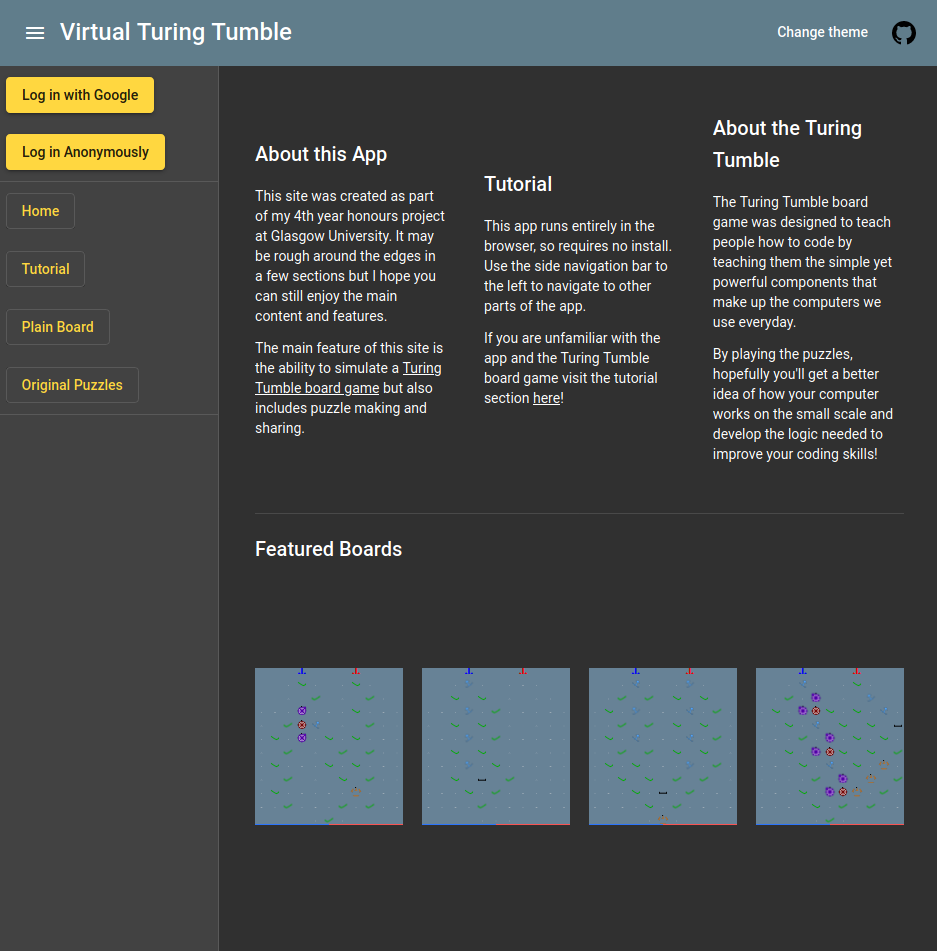
\includegraphics[width=\textwidth]{images/darkTheme.png}
            \caption{Home page with the dark theme}
            \label{fig:homepageDark}
        \end{subfigure}
        \begin{subfigure}[b]{0.7\textwidth}
            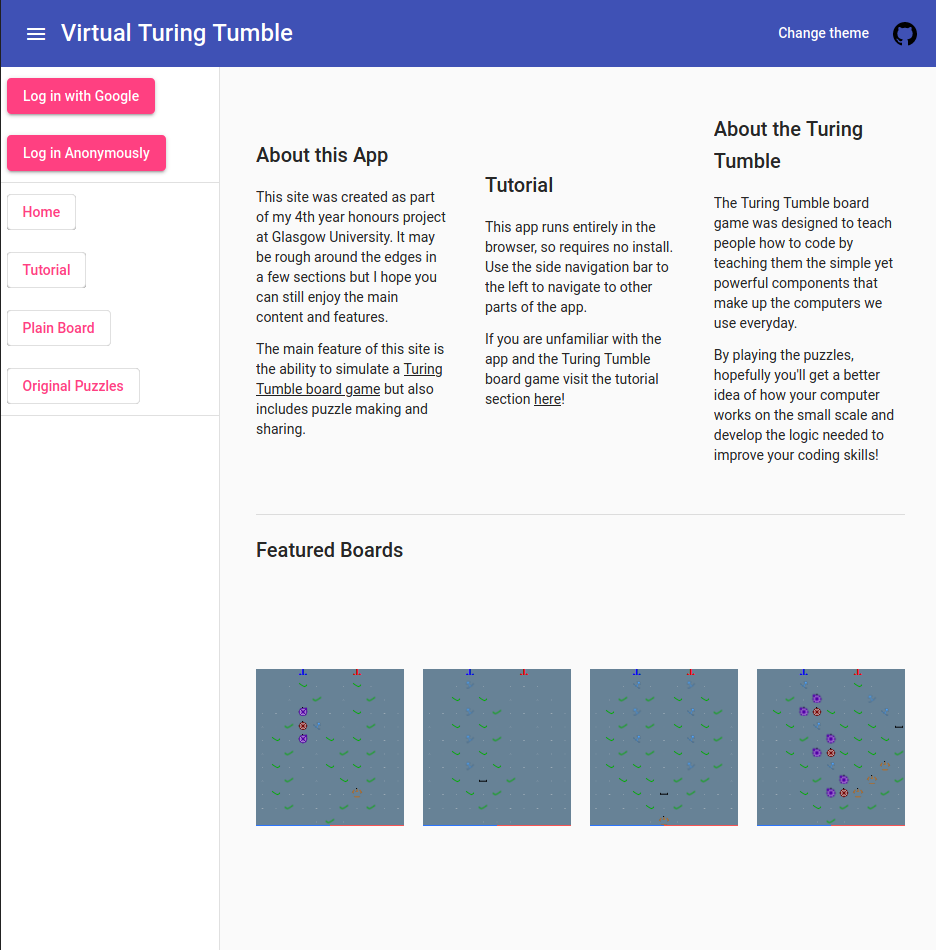
\includegraphics[width=\textwidth]{images/lightTheme.png}
            \caption{Home page with the light theme}
            \label{fig:homepageLight}
        \end{subfigure}
        \caption{The 2 themes are displayed on the home page of the site with the side navigation bar extended}
        \label{fig:themes}
    \end{figure}

    \begin{figure}
    \centering
    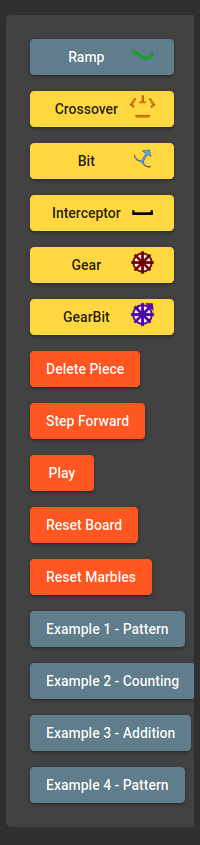
\includegraphics[width=0.2\linewidth]{images/selectionBar.png}
    \caption{The selection bar component when a user is holding a Bit piece}
    \label{fig:selectionBar}
\end{figure}
    
\end{appendices}

%==================================================================================================================================
%   BIBLIOGRAPHY   

% The bibliography style is abbrvnat
% The bibliography always appears last, after the appendices.

\bibliographystyle{abbrvnat}

\bibliography{l4proj}

\end{document}
